\section{Motivation}\label{sec:motivation_md_2022}
As discussed in the previous chapter, PyHEADTAIL simulations including the SPS impedance model suggest that the beam coupling impedance leads to an effective suppression of the $\CC$ RF phase noise induced emittance growth through the separation of the coherent tune from the incoherent spectrum. This suppression, which is related to the coherent (dipole) motion, can reach up to a factor of 4-5 for the experimental conditions of the first experimental campaign with $\CC$s that took place in the SPS in 2018, which seems to be the explanation for the experimental observations (see Section~\ref{sec:MD5_overview}).

This suppression effect has never been observed before. To this end, another experimental campaign took place in the SPS in 2022 where the main objective was to validate experimentally the above-mentioned suggested emittance growth suppression mechanism. If successful, it would constitute the first experimental investigation and validation of this effect. Moreover, achieving a good understanding of the 2018 results is essential for developing confidence in the theoretical model and its predictions for the HL-LHC.

The experimental campaign of 2022 was organised in two proof-of-concept experiments. The first experiment was carried out in the presence of phase noise in the $\CC$ RF system. The second experiment took place with a pure dipolar noise source: the beam transverse damper. This chapter reports on the preparation, the methodology, and the results of these experiments.

\section{Experiment with CC as noise source}\label{sec:cc_md_2022}
Due to the preceding PyHEADTAIL simulations which provided strong evidence that the observed discrepancy between the 2018 measurements and the theoretical predictions could be explained by the beam transverse impedance additional machine time was dedicated to emittance growth studies with $\CC$ in the SPS in 2022. The time allocated for the $\CC$ experiment was limited to about 10 hours since many different studies have to take place in the SPS during the year. Taking into consideration the time needed for the setup and the $\CC$ calibration the time available for the emittance growth measurements is reduced even more. To this end, measurement repeatability is limited and the experimental procedure had to be carefully planned in advance.
% Also you can add that each point in the emittance growth studies needs about 30-40 min.

\subsection{Machine and beam configuration}\label{sec:cc_md_2022_parameters}
The emittance growth measurements in 2022 were performed in "coast" mode at 270\,GeV following the same setup as in 2018 (see Section~\ref{sec:exp_setup_2018}) and very similar machine and beam conditions. The most relevant parameters are listed in Table~\ref{tab:machine_beam_param_2022}. 

The linear chromaticity was corrected to about zero units in both the horizontal and vertical planes. That was a result of miscommunication with the operator team of the SPS machine as the desired value was between 0.5 and 1.0. However, the analysis of the PyHEADTAIL simulations in Section~\ref{subsec:chroma_scan} showed that the sensitivity of the emittance growth suppression to the linear chromaticity values (for small positive values) is expected to be insignificant. 

On the grounds that the last three (out of four) bunches used in 2018 expereimental campain were unstable, in 2022 the experiment was carried out with a single bunch. This choice allowed also to have better control on the beam conditions, avoiding possible effects from interactions between the bunches \footnote{Even though these effects should be insignificant due to the large bunch spacing, see Table~\ref{tab:machine_beam_param_2018}.}.

\begin{table}[!hbt]
	\begin{minipage}{\textwidth}
      \begin{centering}
   \caption{Main machine and beam parameters for the emittance growth studies with CCs in SPS in 2022.}
	\begin{tabu} to \textwidth {X[c,m] X[0.5c,m] X[0.5c,m] X[0.01c,m]}
		&&& \\[-6mm]
		\toprule \toprule
		\multicolumn{2}{l}{\textbf{Parameter}} &
		\multicolumn{2}{c}{\textbf{Value}} \\
		\bottomrule
      \multicolumn{2}{l}{Beam energy, $\symE$} & \multicolumn{2}{c}{270\,GeV} \\
      \multicolumn{2}{l}{Main RF voltage / frequency,  $\VRF$ / $\fRF$}  & \multicolumn{2}{c}{5\,MV / 200.39\,MHz} \\ %200.3945
      \multicolumn{2}{l}{Horizontal / vertical betatron tune, $\Qx$ / $\Qy$}  & \multicolumn{2}{c}{26.13 / 26.18} \\
      \multicolumn{2}{l}{Horizontal / vertical first order chromaticity, $\Qpx$ / $\Qpy$}  & \multicolumn{2}{c}{ $\sim$ 0.0-0.5 / $\sim$ 0.0-0.5} \\
      \multicolumn{2}{l}{Synchrotron tune, $Q_s$}  & \multicolumn{2}{c}{0.0051} \\
      \multicolumn{2}{l}{$\CC 1$ voltage / frequency, $\VCC$ / $\fCC$}  & \multicolumn{2}{c}{1\,MV / 400.78\,MHz} \\
      \multicolumn{2}{l}{Number of protons per bunch, $\Nb$} & \multicolumn{2}{c}{3 $\times 10^{10}$ p/b$^\ast$} \\
      \multicolumn{2}{l}{Number of bunches}  & \multicolumn{2}{c}{1} \\
      \multicolumn{2}{l}{Bunch length, 4$\sigmat$}  & \multicolumn{2}{c}{1.83 \,ns$^\ast$}\\
      \multicolumn{2}{l}{Horizontal / vertical normalised emittance, $\emitx$ / $\emity$}  & \multicolumn{2}{c}{2\,$\mathrm{\mu m}$ / 2\,$\mathrm{\mu m^\ast}$}\\
      \multicolumn{2}{l}{Horizontal / vertical rms tune spread, $\Dqxrms$ / $\Dqyrms$}  & \multicolumn{2}{c}{2.02 $\times 10^{-5}$ / 2.17 $\times 10^{-5}$ $^\ddagger$}\\
      \bottomrule
	\end{tabu}
   \label{tab:machine_beam_param_2022}
   \end{centering} \footnotesize{$^\ast$ These values corresponds to the requested intial value at the start of each coast.  \\ $^\dagger$ This value corresponds to the average rms measured bunch length over all the coasts of 2022. \\$^\ddagger$ Here the rms betatron tune spread includes only the contribution from the detuning with amplitude present in the SPS machine. More details along with the calculations for the listed values can be found in Appendix~\ref{app:detuning_with_amplitude}.}
   \end{minipage}
\end{table}
% For bunch length: cernbox/2022/SPS_MDs_2022/cc_md_16May2022/longitudinal_profiles/visualise_pickle.ipynb

The average bunch length (over all settings) was measured to be about $4\sigma_t$ = 1.83\,ns. During the coasts, an increase in the bunch length of $\sim$5~$\%/h$ on average for each setting was observed. This small increase agrees with what is usually observed in the SPS in coast and will not be taken into consideration in the following analysis. The individual plots illustrating the evolution of the bunch length as measured with the Wall Current Monitor (introduced in Section~\ref{sec:ABWLM_WallCurrentMonitor}) during the experiment are presented in Appendix~\ref{sec:bunch_length_measurements_2022}. Finally, looking at the dependence of the emittance growth suppression by the impedance on the bunch length in Fig.~\ref{fig:study_10_bunch_length} it is evident that the bunch length of $4\sigma_t$ = 1.83\,ns belongs to the regime of the strong suppression. This is important as it optimizies the experimental conditions to observe the impedance effects on the noise-induced emittance growth. \textcolor{red}{The last sentence needs to be refined. See comment from Any.}

The intensity was set to $3 \times 10^{10}$ protons to be in agreement with the experiment of 2018. During the coasts of the 2022 experiment almost zero losses were observed. Therefore, the evolution of the intensity during the coasts will be not considered in the following.


\textbf{CC RF noise}\\
The noise injected in the $\CC$ RF system was again a mixture of phase and amplitude noise. The noise excitation extended from DC up to 10\,kHz and thus the noise was applied on the first betatron sideband only, at $\sim$8\,kHz. The PSD values at $\sim$8\,kHz of the four different levels of artificial noise that were used in the experiment are listed in Table~\ref{tab:noise_settings_2022}. By looking at the table, it becomes evident that the contribution of amplitude noise to the total emittance growth was found to be small (about 7$\%$). To this end, in the post-processing of the 2022 data, the introduction of the effective phase noise (see Section~\ref{sec:injected_RF_noise}) is not required. In the following, the measured growth rates will be displayed as a function of the measured RF phase noise only. This choice is also justified by the fact that the objective of the 2022 experimental campaign with $\CC$s is to mainly reproduce the qualitative expected bahevior from the impedance and not the exact values. This is discussed further in the next sections of this chapter.

% I don't have the data to plot the spectra. Only screenshots in the logbook.


% Note 1: Noise level values from the logbook.
% Note 2: Analysis and percentages: /2022/SPS_MDs_2022/cc_md_16May2022/roundA_online_analysis_ws/summary_plots/for_thesis/cc_md_analysis_noise_scan_for_thesis.ipynb
\begin{table}[!hbt]
	\centering
   \caption{Phase and amplitude noise levels injected in the CC RF system for the emittance growth studies of 2022 along with the analytically expected growths. The listed noise values correspond to the PSD values at the first betatron sideband, $f_b$, at $\sim$8\,kHz. The analytical emittance growth rates were computed using Eq.~\eqref{eq:dey_an} and~\eqref{eq:dey_pn} for bunch length of $4\sigma_t$=1.83\,ns.}
	\begin{tabu} to \textwidth { X[c,m] X[c,m] X[c,m] X[c,m] X[c,m]}
		&&&& \\[-6mm]
		\toprule \toprule
		\multicolumn{1}{l}{} &
		\multicolumn{2}{c}{$\mathbf{10\,\boldsymbol{\log}_{10} \mathcal{L}(f)}$ \textbf{[dBc/Hz]}} & \multicolumn{2}{c}{\textbf{Analytical } $\mathbf{d \boldsymbol{\epsilon}_y/dt \ [\boldsymbol{\mu} m/h]}$} \\
		\bottomrule
      \multicolumn{1}{l}{} & 	\multicolumn{1}{c}{\textbf{Phase noise}} & \multicolumn{1}{c}{\textbf{Amplitude noise}} & \multicolumn{1}{c}{\textbf{Phase noise}} & \multicolumn{1}{c}{\textbf{Amplitude noise}} \\
      \midrule
      \multicolumn{1}{l}{Level 1}  & \multicolumn{1}{c}{-115.2} & \multicolumn{1}{c}{-124.6} & \multicolumn{1}{c}{1.64} & \multicolumn{1}{c}{0.16} \\
      
      \multicolumn{1}{l}{Level 2}  & \multicolumn{1}{c}{-109.5} & \multicolumn{1}{c}{-120.5} & \multicolumn{1}{c}{6.11} & \multicolumn{1}{c}{0.42}\\

      \multicolumn{1}{l}{Level 3}  & \multicolumn{1}{c}{-104.7} & \multicolumn{1}{c}{-116.0} & \multicolumn{1}{c}{18.44} & \multicolumn{1}{c}{1.19} \\

      \multicolumn{1}{l}{Level 4}  & \multicolumn{1}{c}{-100.1} & \multicolumn{1}{c}{-111.0} & \multicolumn{1}{c}{53.19} & \multicolumn{1}{c}{3.76} \\ 
      \arrayrulecolor{black}\bottomrule
	\end{tabu}
   \label{tab:noise_settings_2022}
\end{table}



\textbf{CC1 instead of CC2}\\
In the 2022 campaign, $\CC$1 was used instead of $\CC$2 which was used in 2018. The reason behind this is that during the phase offset scan performed for the calibration of the $\CC$ module (details on the procedure can be found in ... section in chapter 4 and  Section~\ref{subsec:cc_calibration_2022}) $\CC$2 tripped systematically. The issue is associated with the change of the RF phase but fixing this problem would have been time-consuming which was not an option due to the very limited machine time of the MD. Therefore, for the measurements in 2022 $\CC$1 was used.
% CC2 tripped: see the entry of the logbook 4/5/2022, at 11:30:30 

\textbf{SPS Wire Scanners}\\
The emittance values were measured with the SPS Wire Scanners according to the procedure discussed in Section~\ref{subsec:sps_ws}. In particular, wire scanners SPS.BWS.51637.H and SPS.BWS.41677.V were used for measurements in the horizontal and vertical planes, respectively. For both devices the data points from the second photomultiplier were used (PM2) \footnote{Each Wire Scanner device is equipped with four PMs. Each one of them provides a better resolution of the amplitude signal of the secondary particles for a different regime. The choice of PM2 for the emittance growth studies in 2022 was done "online", during the experiment, by examining the obtained beam profiles.}. The beta functions of the respective plane at the locations of the wire scanners are 79.29\,m, and  60.75\,m. 
% The values of the beta functions were obtained from MADX: https://github.com/natriant/exploring_SPS/blob/master/madx_studies/optics_new_seq_after_LS2/output/twiss_thin_elements/find_beta_functions_at_locations.ipynb 

As explained erlier (see Section~\ref{subsec:sps_ws}) during each measurement with the wire scanners the beam profile is acquired two times as the wire crosses the beam in the forward direction (IN scan) and then in the reverse direction (OUT scan). For the experiment of 2022, the OUT scan was performed just 200\,ms after the IN scan. However, it was observed that there are significant discrepancies between the measurements from IN and OUT scan, which in some cases reached up to 1\,$\mathrm{\mu m}$. By looking at the acquired profiles no reason was found to exclude or not one of the two scans. A significant effort was done with the wire scanner experts during the emittance growth experiment trying to mitigate this effect without success due to limitations on the hardware of the current instrument. Therefore, it was decided that the post-process analysis would be performed taking into account only the IN scan measurements since they appeared to have systematically less fluctuation than in the OUT scan.

It is worth commenting that this issue was not observed in the 2018 measurements. A possible explanation is that the wire scanner acquisitions of 2022 provide lower number of points to reconstruct the bunch profiles (compare Figs.~\ref{fig:WS_example_V_profile} against~\ref{fig:WS_example_profiles_V_2022}) increasing the uncertainty of the obtained emittances. The reason behind this, is that between 2018 and 2022 the wire scanners had undergone an upgrade which increased their speed while crossing the bunch. A possible solution to this issue would be to reduce the speed of the wire for the emittance growth experiments in "coast" mode. This is currently in discussion with the team responsible for the wire scanners of the SPS.

% Evidence for the strong difference between IN and OUT https://docs.google.com/presentation/d/1QIaQNfqVWaI8cHGGgb5eeS7c_jdUMuxLqD_poHrOtH0/edit?usp=sharing

Last, the low emittance growth rates showed a significant sensitivity to the fluctuation of the wire scanner measurements. For this reason, for the low $\CC$ noise levels, long measurement times of about 30-40 minutes were needed.


\textbf{Head-Tail monitor calibration}\\
From the end of 2018 till the end of 2020, the CERN accelerator complex has undergone its second long shutdown in order to complete its scheduled upgrade program. Therefore, the calibration of the HT monitor was repeated to provide the normalisation factor required for the scaling of its reading (see Section~\ref{subsec:HT_post_process_CC}). The calibration factor was found to be 0.1037 in November 2021, as shown in Fig.~\ref{fig:HT_calibration_2022_levens} (slope value).

\begin{figure}[!h] % Email communication with T. Levens on 8 November 2021.
    \centering         
    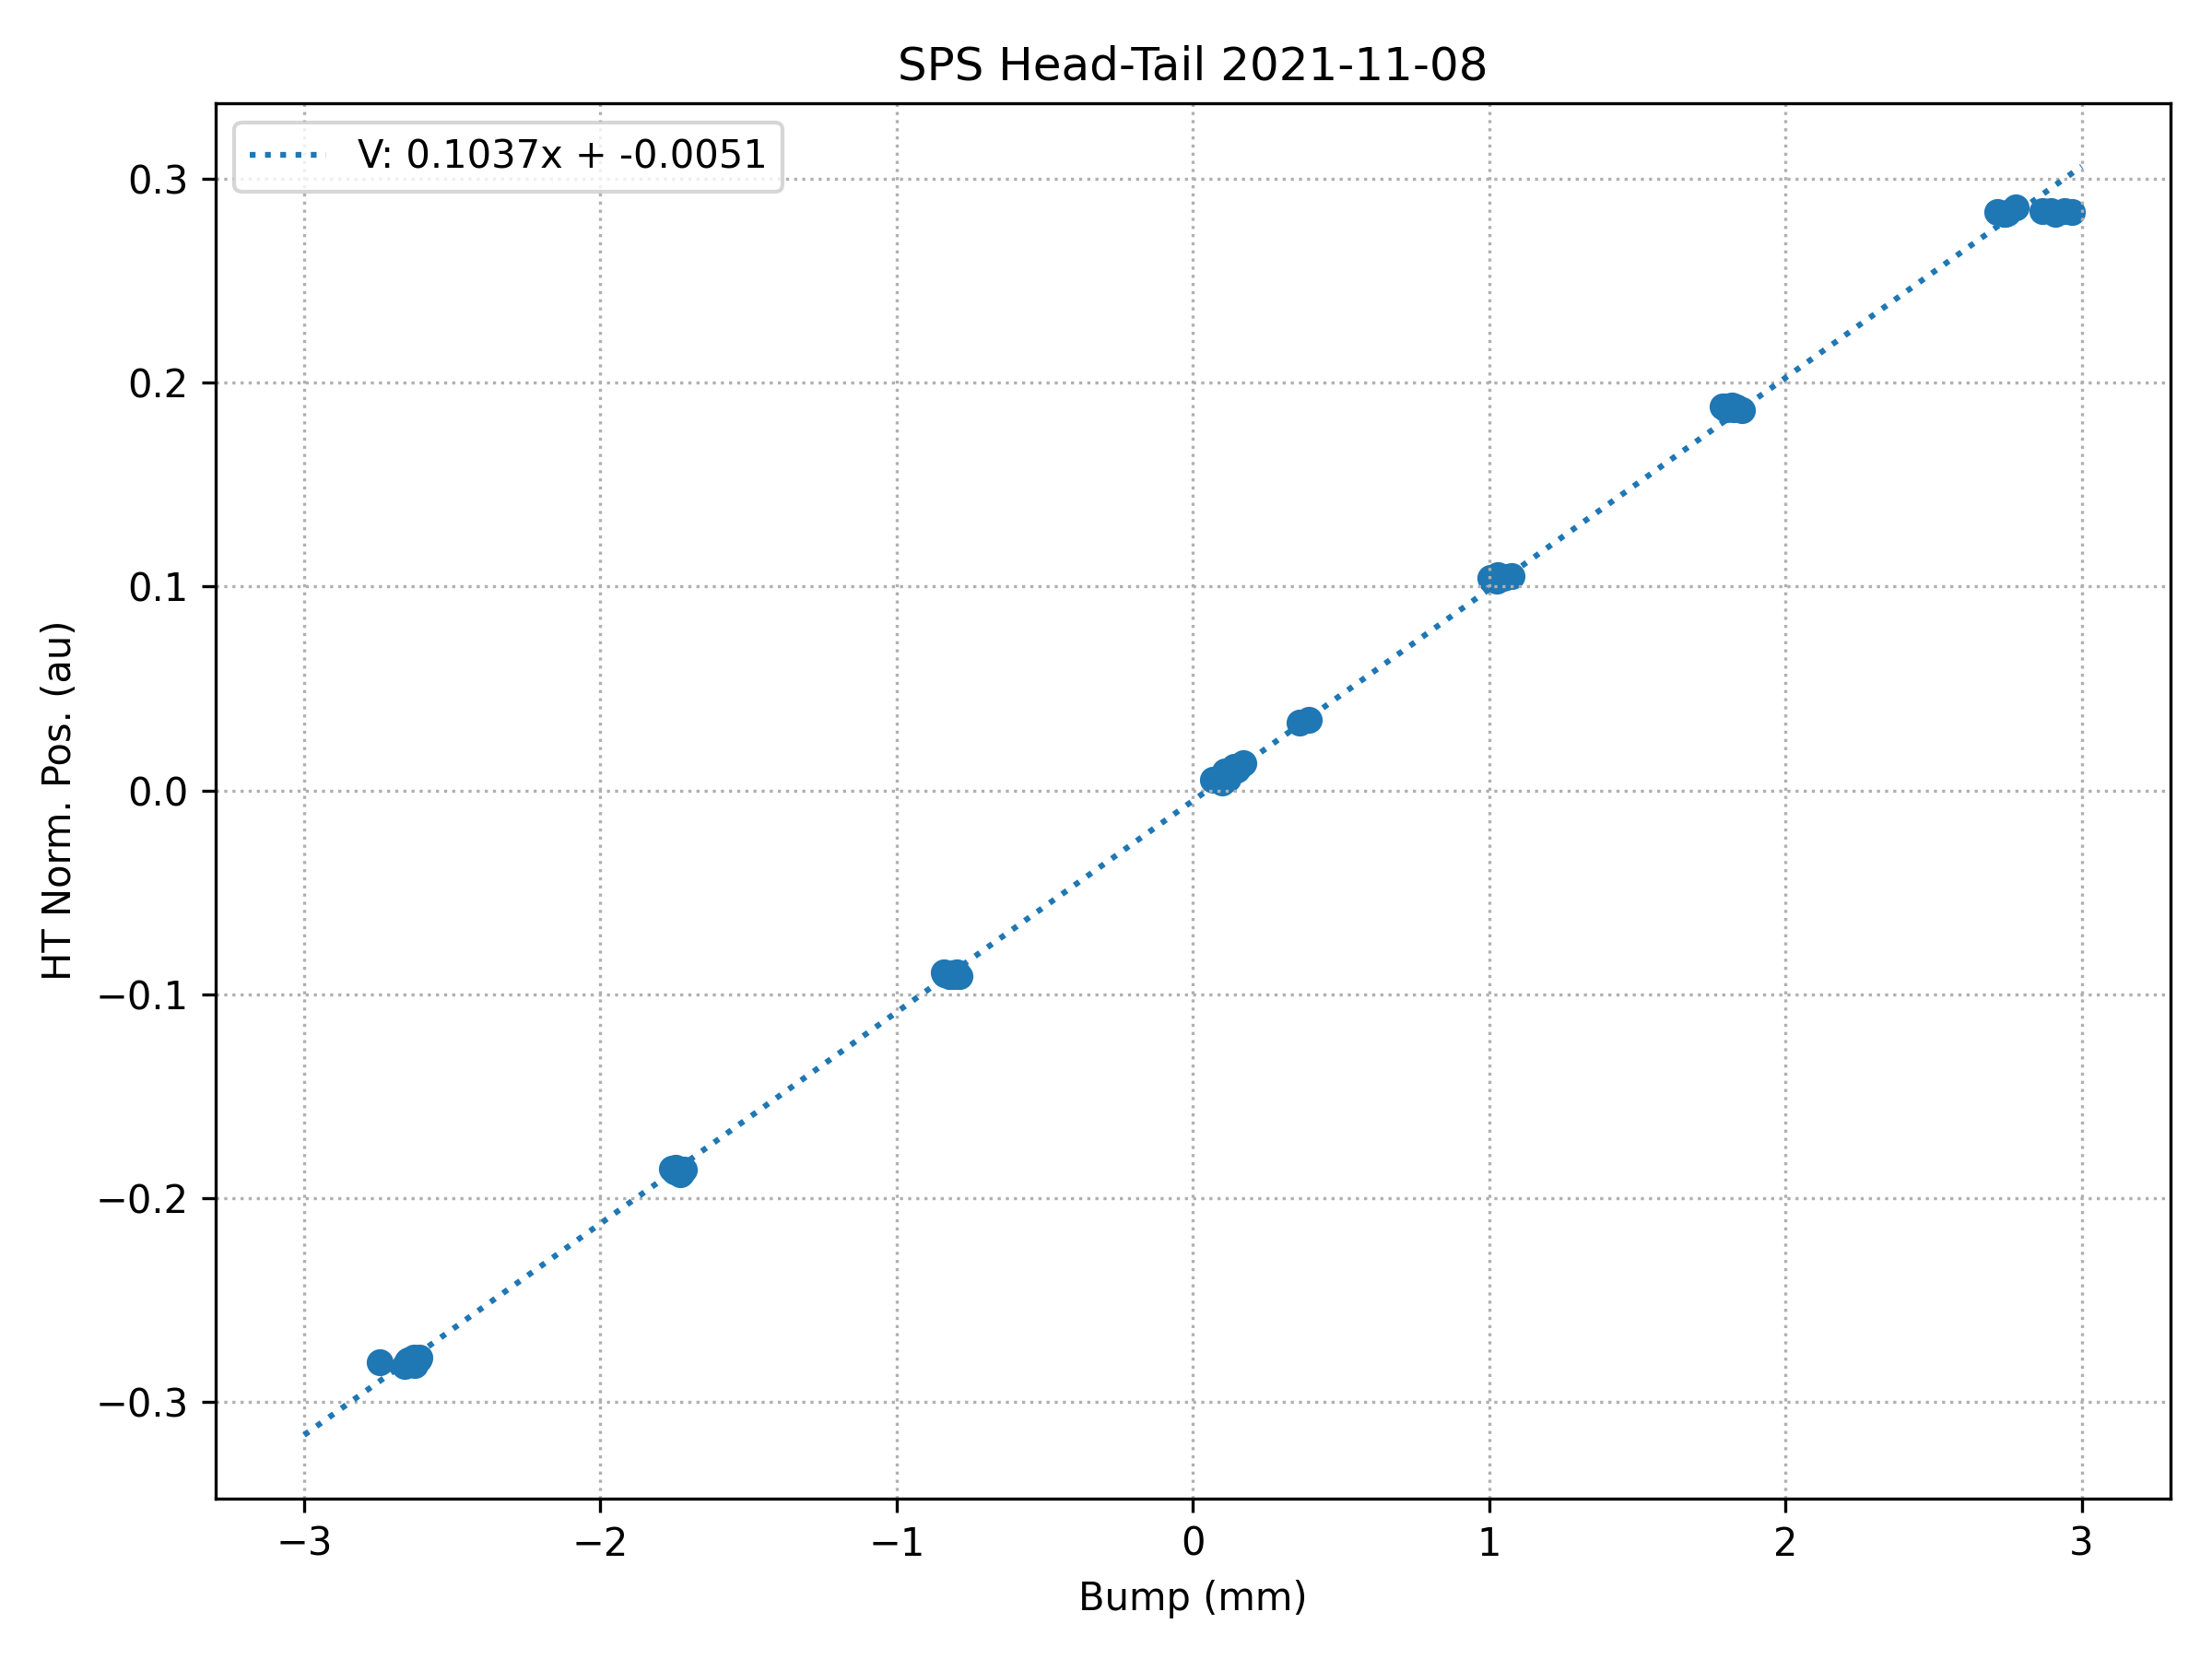
\includegraphics[width=0.7\textwidth]{images/Ch8/HT_monitor_calibration_2022.png}
        \caption{The calibration was performed by T.~Levens by performing orbit bumps (around the reference orbit) and measuring the normalised position of the bunch in the vertical plane (plane of interest). The normalised position is obtained as the difference of the signal divided by the sum. More details on the calibration procedure are given in Ref.~\cite{PhysRevAccelBeams.22.112803}. This plot is courtesy of T.~Levens .}
        \label{fig:HT_calibration_2022_levens}
 \end{figure}


\subsection{Experiment preparation and procedure}\label{sec:cc_md_2022_preparation}
\textbf{Objectives}\\
The available machine time ($\sim$ 10 hours) for the $\CC$ experiment of 2022 was split into two parts. For the first part, the objective was to measure the emittance growth with the same noise levels and conditions as in 2018 in order a) to reproduce the observed scaling of emittance growth (see Fig.~\ref{fig:MD5_summary_plot}) and b) to benchmark the expected suppression factor from PyHEADTAIL simulations with the impedance model. This will be referred to as $\CC$ Experiment A in the following.

The objective of the second part was to investigate the effects of impedance and amplitude detuning on the emittance growth from $\CC$ phase noise. The preceding analysis of the PyHEADTAIL simulations revealed a significant sensitivity of the emittance growth suppression on amplitude-dependent tune shift (e.g. Fig.~\ref{fig:MD_2018_impedance_simulations}). This behavior can be tested experimentally in the SPS with the use of the Landau octupole families, which allow for the introduction of controlled detuning with amplitude. A successful reproduction of this behavior would provide the proof-of-concept for the emittance growth suppression mechanism from the beam transverse impedance. This will be referred to as $\CC$ Experiment B in the following. It should be mentioned, that for this experiment the octupoles of the LOD family are employed as they act mostly in the vertical plane which is the plane of interest in this studies (vertical $\CC$ module which results in vertical emittance growth).

\textbf{Preparatory studies with PyHEADTAIL simulations}\\
In preparation for the $\CC$ experiments (A and B) the emittance growth in the presence of $\CC$ RF phase noise was simulated with PyHEADTAIL including the most up-to-date SPS impedance model~\cite{updated_sps_wakfields_model} as a function of different octupole strengths, $k_{\mathrm{LOD}}$. The beam and machine parameters are the ones reported in Table~\ref{tab:machine_beam_param_2022} which correspond to the experimental conditions of 2022. The emittance growth is induced by $\CC$ RF phase noise with a power spectral density of 1.68\,$\mathrm{rad^2/Hz}$ in the first betatron sideband which results in an emittance growth rate of about 25\,nm/s. It should be highlighted that this noise level is much stronger than the levels of the injected artificial noise used in the experiment, in order for the growth to be easily observed in the simulation time of just 2.5\,s. Therefore, the goal of the experiments was to reproduce the simulated suppression factor and behavior only and not the exact numbers. Finally, the simulation setup and the $\CC$ RF phase noise were simulated as discussed in Chapter~\ref{Ch:suppression_impedance}. 

The emittance growth was simulated over a range of twenty one $k_\mathrm{LOD}$ values equally spaced from -28.2\,$\mathrm{1/m^4}$ to +28.3\,$\mathrm{1/m^4}$. Nevertheless, in the simulations, no actual octupolar elements were used in order to avoid the excitation of resonances as discussed in Section~\ref{sec:first_obs_suppression}. Instead, following the preceding PyHEADTAIL simulations, the effect of LODs is introduced as a change in the phase advance of the individual particles depending on their individual actions and defined by the corresponding detuning coefficients. The study was performed for zero horizontal detuning coefficient, $\alpha_{xx}$=0 while the values of the vertical, $\alpha_{yy}$, and the cross-term, $\alpha_{yx}$, coefficients were estimated using MAD-X~\cite{madx}.

Figure~\ref{fig:pyheadtail_cc_impedance_2022_md_octupole_current} illustrates the dependence of the $\CC$ RF phase noise-induced emittance growth on the LOD strength, in the absence (blue) and the presence (orange) of the wakefields. The analytical prediction of the model Mastoridis--Baudrenghien is also given to facilitate the identification of the suppression factor from the impedance (horizontal black dashed line). As usual, in the absence of wakefields, there is a very good agreement between the simulation results and the theoretical predictions. In the presence of wakefields, the expected dependence on the tune spread appears. The rms tune spread values (shown on the secondary horizontal axis) are computed taking into account both the $\alpha_{\mathrm{yy}}$ and $\alpha_{\mathrm{yx}}$ coefficients using Eq.~\eqref{eq:rms_amplitute_detuning_3}.

% 1) Slides on computing the octupole current: https://docs.google.com/presentation/d/1VgGMqCevej4Eh7bjdGFSEPVI0zLxqB2S5FxLtFGhp2I/edit#slide=id.ge970b2a80a_0_16
The green and yellow areas indicate regimes where the octupoles require less than 200\,A and 400\,A respectively for their operation. The maximum operational current for the LODs in SPS is 400\,A. However, due to their planned continuous operation in multiple coasts, the LOD current should stay below 200\,A. The required current for the octupoles is computed from their strength, $k_\mathrm{LOD}$, using Eq.~\eqref{eq:I_vs_B3_relation_lof}


% /eos/user/n/natriant/pyheadtail_data/final_for_thesis/2022_conditions/CC1/deyRates_sps_270GeV_PN1e-8_400MHz_SPS_CC2_updatedWakes_y-plane_WakesOFF_vs_WakesON_new_QpxQpy0.5_6D_Nb5e5_intensity3e10Scan_vs_TuneSpreadvsExpectedSPS_octupole_current.png
\begin{figure}[!h] % Email communication with T. Levens on 8 November 2021.
   \centering         
   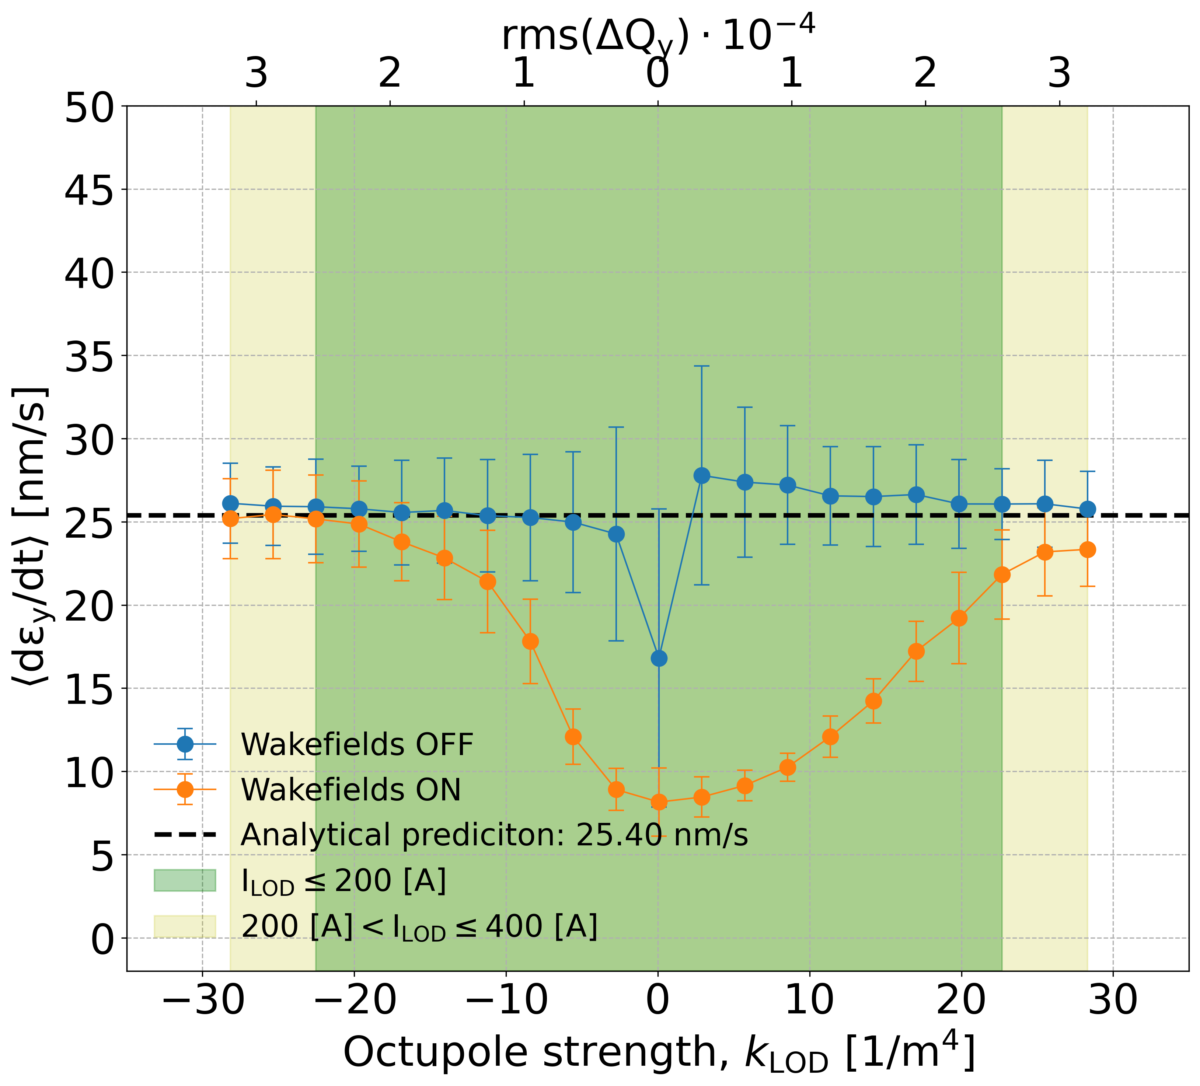
\includegraphics[width=0.8\textwidth]{images/Ch8/deyRates_sps_270GeV_PN1e-8_400MHz_SPS_NewWakesAllcontributions_appendWakes_y-plane_WakesONvsOFF_QpxQpy1_6D_Nb5e5_intensity3e10Scan_vs_TuneSpreadvsExpectedSPS_octupole_current.png}
       \caption{Transvserse emittance growth driven by CC RF phase noise without (blue) and with (orange) the impedance effects. The green and yellow areas indicate regimes where the octupoles require less than 200\,A and 400\,A respectively for their operation.}
       \label{fig:pyheadtail_cc_impedance_2022_md_octupole_current}
\end{figure}

From Fig.~\ref{fig:pyheadtail_cc_impedance_2022_md_octupole_current}, we make the following observations:
\begin{enumerate}
   \item The asymmetry in the suppression factor for positive and negative detuning with amplitude observed in the simulations for the 2018 experimental conditions (Chapter~\ref{Ch:suppression_impedance}) seems to be mitigated here. Nevertheless, in order to exit the suppression region the negative polarity of the octupoles (LOD) should be preferred.
   \item Without powering the octupoles (2018 conditions), $k_\mathrm{LOD}$=0, a suppression of a factor of about 3 is observed.
   \item Even for the strongest octupole strengths, $| k_\mathrm{LOD} |\approx 30 \ \mathrm{/m^4}$, the required current remains below 400\,A. Consequently, no crucial limitations are introduced to the experiment from the octupoles operation.
\end{enumerate}

\textbf{Experimental procedure}\\
The experiment was carried out on 16 May 2022, from 09:15 to 18:40. The steps taken during the experimental study were the following:

\begin{enumerate}
   \item Calibration of the voltage and phase offset of the CC.
   \item Measurement of the background growth rate in "coast" mode: CC is switched on but with no additional noise injected in its RF system and the Landau octupoles switched OFF.
   \item Measurement of the emittance growth with the Landau octupoles switched OFF and for four different $\CC$ noise levels as in 2018 (CC Experiment A). For each noise level a new bunch was injected.
   \item Measurement of the emittance growth for a selected noise level and varying octupole strength (CC Experiment B). For each octupole setting a new bunch was injected in the SPS.
\end{enumerate}


The details and the results of the above mentioned steps will be presented in the following subsections.

\subsection{Calibration of CC voltage and phase offset}\label{subsec:cc_calibration_2022}
The first step in the CC experiment was to calibrate its voltage and phase offset. The calibration took place following the procedure described in Section... at 270\,GeV and it lasted for about 15 minutes (start: $\sim$09:40, end: $\sim$09:52).

To provide an overview, the calibration was performed by varying the inspector \textcolor{red}{(add here cross reference to chapter 4 where the term inspector is explained)} phase of CC1 from -180$^\circ$ to +180$^\circ$ in steps of 30$^\circ$. For each step, the crabbing signal was acquired with the HT monitor and the CC voltage signal was reconstructed. For each acquisition, the $\CC$ voltage at the center of the bunch, $t=0$, was plotted as a function of the corresponding inspector phase. The results of the inspector phase scan for $\CC$1 are summarised in Fig.~\ref{fig:Vcc_calibration_md_2022}.

\begin{figure}[!h] % /eos/user/n/natriant/2022/SPS_MDs_2022/cc_md_16May2022/HT_monitor_phase_CC_offset_calibration
   \centering         
   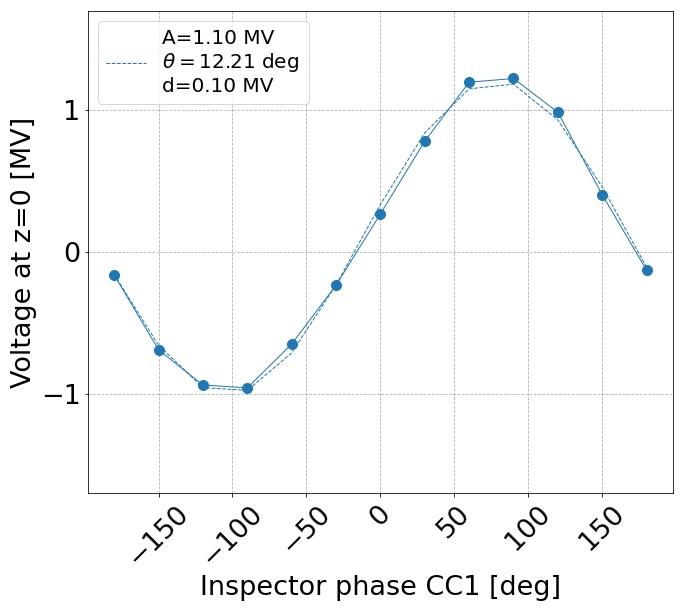
\includegraphics[width=0.7\textwidth]{images/Ch8/Vcc_at_z_zero_vs_inspector_phase_CC1_for_thesis.png}
       \caption{Calibration plot for the CC1 as obtained during the experiment on 16 May 2022, displaying the CC voltage at the center of the cavity $t=0$ for different values of the inspector phase.}
       \label{fig:Vcc_calibration_md_2022}
\end{figure}

From the beam based measurements with the HT monitor the voltage of CC1 was found to be 1.1\,MV, very close to the targeted one (1\,MV). The phase offset was found to be 12.21$^\circ$. For the rest of the experiment, inspector phase was set to the opposite of the phase offset so that the CC phase is zero.

Between $\sim$11:39 and $\sim$11:45 the same scan for CC2 was attempted. However, the cavity tripped systematically due to issues associated with the change of the RF phase. Fixing this issue would have been time-consuming, and was not possible due to the very limited machine time of the MD. Therefore, for the measurements in 2022 $\CC$1 was used.
% CC2 tripped: see the entry of the logbook 4/5/2022, at 11:30:30 

\subsection{Measurement of background growth rate in "coast" mode}\label{subsec:measured_background_growth_cc_md_2022}
After the calibration of CC1, the coast at 270\,GeV was set up for the emittance growth measurements. First, the background emittance growth, with no additional noise injected in the CC and the Landau octupoles switched off was measured. The background emittance growth was found to be similar in both transverse planes: $d\epsilon_x /dt$ = 0.81\,$\mathrm{\mu m}$ and $d\epsilon_y /dt$ = 0.84\,$\mathrm{\mu m}$ in the horizontal and vertical planes respectively. This measured background emittance growth is illustrated in Fig~\ref{fig:cc_md_2022_background_growth_in_scan} for both the horizontal (blue) and vertical (red) planes.

\begin{figure}[!h] % /eos/user/n/natriant/2022/SPS_MDs_2022/cc_md_16May2022/roundA_online_analysis_ws/online_analysis_scripts_figures/coast1
   \centering         
   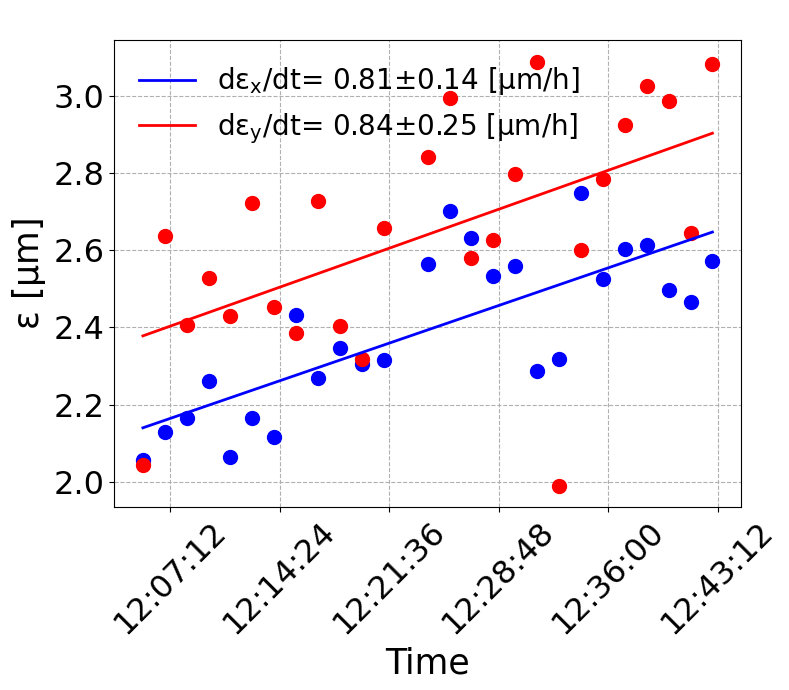
\includegraphics[width=0.7\textwidth]{images/Ch8/cc_md_2022_background_in_scan.png}
       \caption{Horizontal (blue) and vertical (red) background emittance growth measured during the experiment with CC1 in 2022, with no injected artificial noise and with the Landau octupoles switched OFF.}
       \label{fig:cc_md_2022_background_growth_in_scan}
\end{figure}
% There was no valid reason to exclude any of the points even the outliers.

The applications used in the control room for the monitoring of the SPS machine have undergone an upgrade between the years 2018 and 2022. The latest applications which activate the wire scanners and automatically compute the emittance values from the profiles do not compute the respective errors. Nevertheless, the profile measurement data are available and thus the uncertainties of the emittance values can be calculated at a later post-processing stage. This post-processing showed that the uncertainties of the emittance values (computed as shown in Chapter~\ref{Ch:2018_analyisis}) are 2-3 orders of magnitude smaller than the emittance values themselves \footnote{See Appendix~\ref{sec:sps_transverse_beam_profiles}}. Therefore, their impact is insignificant and the uncertainties of the emittance growth rates are dominated by the fluctuation of the Wire Scanner acquisitions. To this end, they are not shown in the emittance growth plot nor included in the fit to facilitate the analysis.

From the above figure, it is evident that there is a significant fluctuation in the emittance values in both transverse planes. By looking at the beam profiles, no evidence (e.g. corrupted profiles, abnormal tails, large errors on the gaussian fit results) was found to exclude some of the points. This fluctuation is introduced by the Wire Scanners used for the measurements. As discussed with the experts it appears to be within the limitations of the instrument for these small emittance values. In order to reduce the sensitivity of the linear fit (from which the emittance growth rates are obtained) longer measurements are required (at least 40 minutes). For larger emittance growth rates, or in other words for larger emittance values, these fluctuations are mitigated. 

Finally, for reference, the "natural" amplitude and phase noise at 8\,kHz were measured to be -130.2\,dBc/Hz and 125.7\,dBc/Hz respectively. The theoretically~\cite{PhysRevSTAB.18.101001} expected emittance growth from those noise levels was 0.05\,$\mathrm{\mu/h}$ and 0.19\,$\mathrm{\mu/h}$ in the horizontal and vertical planes respectively from both noise types combined.
% y-plane --> AN: 0.045 um/h, PN: 0.14 um/h
% x-plane --> AN: 0.002 um/h, PN: 0.05 um/h
% Directory to compute these rates: /afs/cern.ch/work/n/natriant/public/SPS_MDs_2022/cc_md_16May2022/cmpt_emit_growth_theoretical_model
% Also some of the growth in the horizontal plane is expected by the IBS. How much I do not know yet.
The rest of the observed growth rates, is due to other sources which are not yet will identified (see discussion in Chapter~\ref{Ch:2018_analyisis}).

\subsection{Results of CC Experiment A: scaling of emittance growth with noise power}\label{subsec:cc_md_2022_noise_scan}

The objective of the first part of the experiment was to reproduce the scaling of the emittance growth driven by CC RF noise with the noise power as observed in 2018. Four different levels of artificial noise were injected in the RF system of the $\CC$ as listed in Table~\ref{tab:noise_settings_2022} and the emittance evolution was recorded in coast every $\sim$1.5 minute. For each noise level, a new bunch was injected such as all the measurements took place with the same initial conditions. The duration of each coast varied from about 30 minutes for the low noise levels to about 20 minutes for the strong noise. 

For the strong noise, less measurement time is sufficient since the growth rate obtained from the linear fit on the emittance values is not sensitive to the fluctuations due to the Wire Scanner. Additionally, for strong noise, the emittance reaches very quickly very large values, about 8-10\,$\mathrm{\mu m}$, which eventually degrades the quality of the beam.

Figure~\ref{fig:cc_md_2022_overview_plots_noise_scan} illustrates the transverse emittance growth measured in the SPS in 2022 for the four different noise levels injected in the $\CC$ RF system increasing from top left to bottom right. It can be seen, that there is a clear emittance growth in the vertical plane which is faster for stronger noise as expected. A growth in the horizontal emittance is also observed it seems independent from the growth in the vertical. This is also confirmed in Fig.~\ref{fig:H_V_emit_growth_noise_scan} where the vertical and horizontal growth rates are plotted as a function of the four different phase noise levels. Consequently, even though in the 2018 analysis (see Chapter~\ref{Ch:2018_analyisis}) the total emittance growth given by $d\epsilon_y/dt +d\epsilon_x/dt $ was considered to account for coupling effects, in the following of the experimental data (2022) the growth in two planes will be treated independently.


% Note 1, figures: /eos/user/n/natriant/2022/SPS_MDs_2022/cc_md_16May2022/roundA_online_analysis_ws/for_thesis
% Note 2, scripts to plot: /afs/cern.ch/work/n/natriant/public/SPS_MDs_2022/cc_md_16May2022/ws_measurements 
\begin{figure}[htp]
   \centering
   \begin{subfigure}{.45\textwidth}
       \centering
       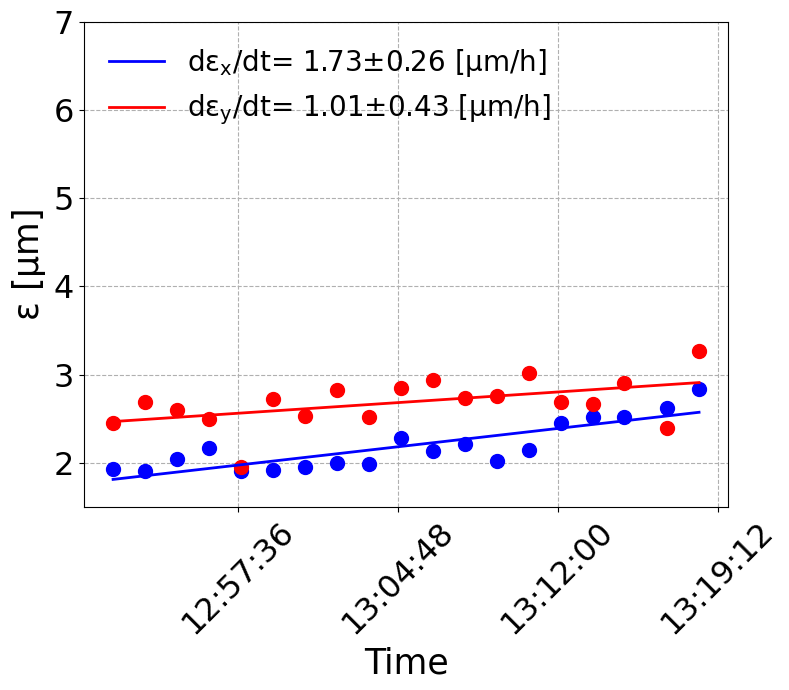
\includegraphics[width=.95\linewidth]{images/Ch8/emit_vs_time_Set1_coast2.png}  
       \caption{-115.2\,dBc/Hz}
       \label{fig:cc_md_2022_coast2}
   \end{subfigure}
   \begin{subfigure}{.45\textwidth}
       \centering
       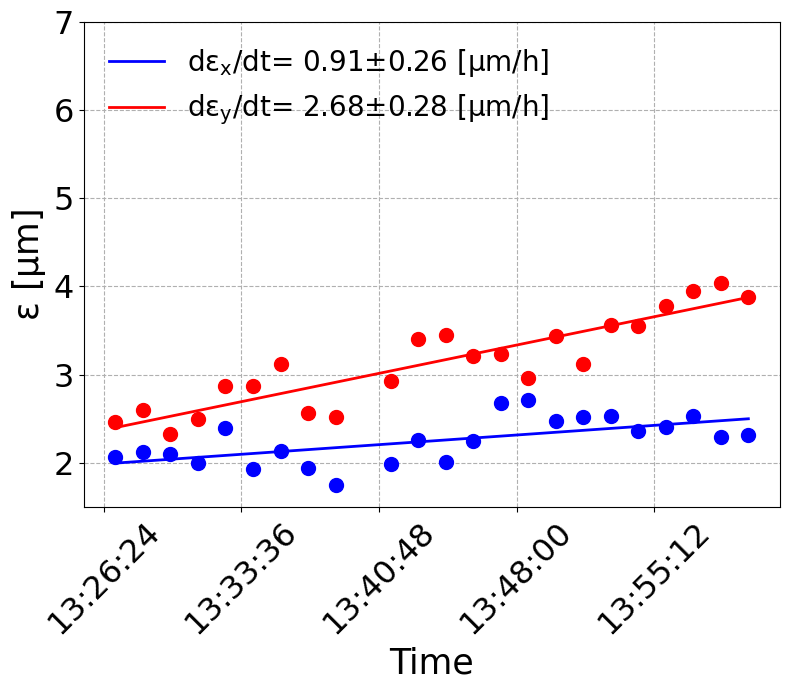
\includegraphics[width=.95\linewidth]{images/Ch8/emit_vs_time_Set1_coast3.png}  
       \caption{-109.5\,dBc/Hz}
       \label{fig:cc_md_2022_coast3}
   \end{subfigure}
   \begin{subfigure}{.45\textwidth}
       \centering
       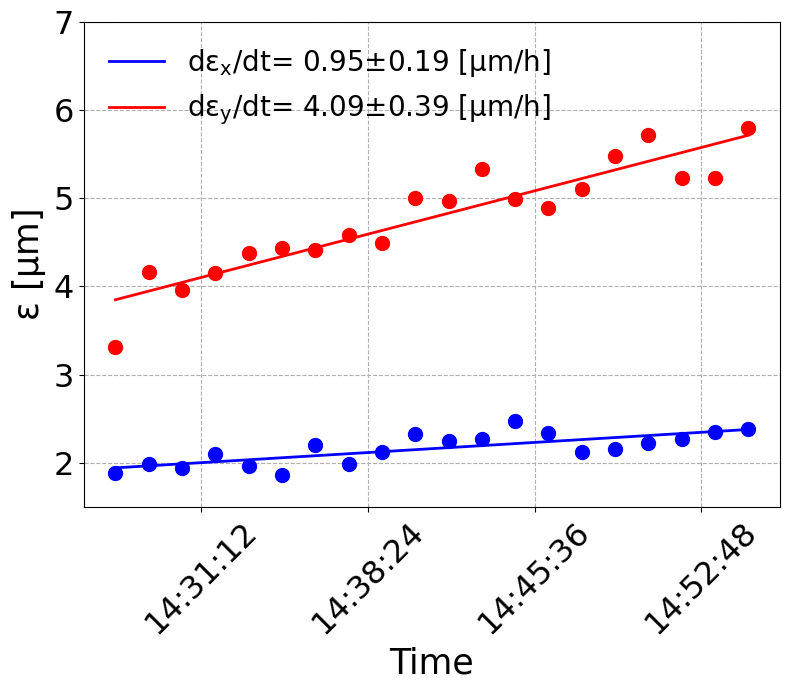
\includegraphics[width=.95\linewidth]{images/Ch8/emit_vs_time_Set1_coast4.png}  
       \caption{-104.7\,dBc/Hz}
       \label{fig:cc_md_2022_coast4}
   \end{subfigure}
   \begin{subfigure}{.45\textwidth}
           \centering
           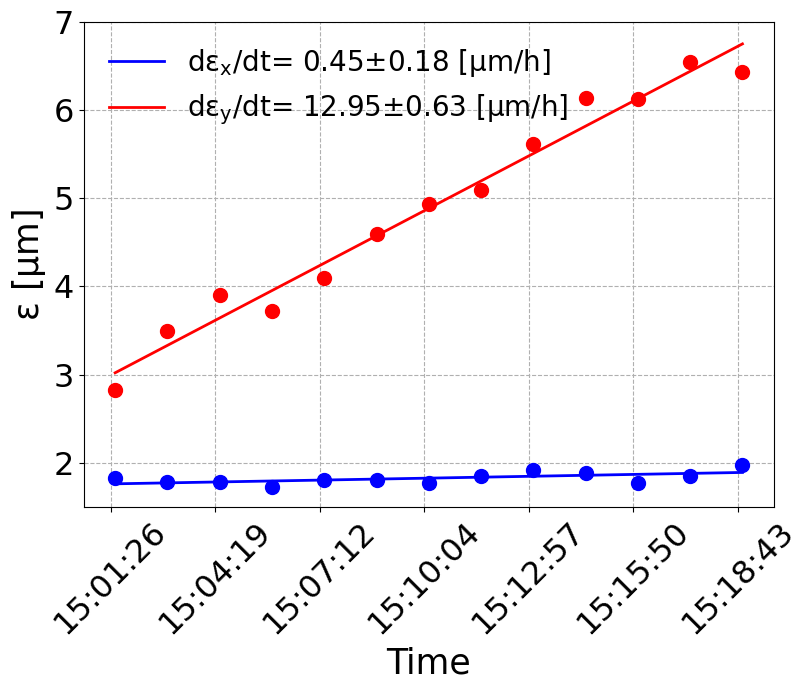
\includegraphics[width=.95\linewidth]{images/Ch8/emit_vs_time_Set1_coast5.png}  
           \caption{-100.1\,dBc/Hz}
           \label{fig:cc_md_2022_coast5}
   \end{subfigure}
   \caption{Horizontal (blue) and vertical (red) emittance evolution of a single bunch during the CC experiment on May 16, 2022. The different phase noise levels injected in the RF system of CC1, are displayed at the captions of each plot.}
   \label{fig:cc_md_2022_overview_plots_noise_scan}
\end{figure}

% Figure: /eos/user/n/natriant/2022/SPS_MDs_2022/cc_md_16May2022/roundA_online_analysis_ws/summary_plots/for_thesis/emit_H_and_V_noise_scan.png
\begin{figure}[!h] 
     \centering         
   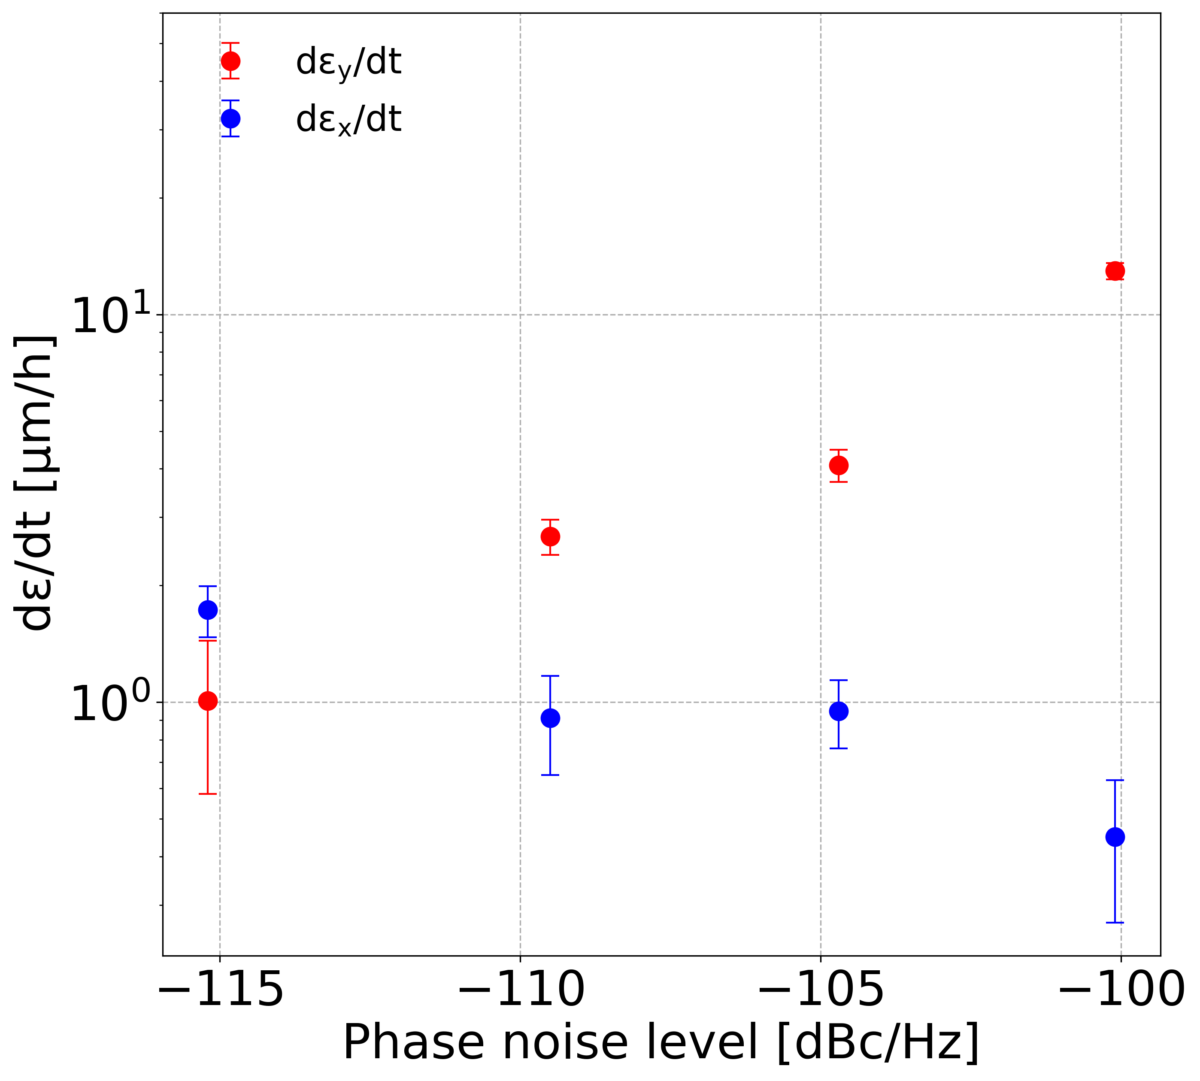
\includegraphics[width=0.7\textwidth]{images/Ch8/emit_H_and_V_noise_scan.png}
       \caption{Overiview plot of the emittance growth study with noise injected in the CC1 in 2022. The measured horizontal (blue) and vertical (red) emittance growth rates are shown as a function of the different phase noise levels of applied noise. The error bars indicate the error of the linear fit on the emittance values (see Section~\ref{sec:emit_growth_meas_2018}).}
       \label{fig:H_V_emit_growth_noise_scan}
\end{figure}


\textbf{Summary plot}\\
Figure~\ref{fig:V_emit_growth_background_subtracted_noise_scan} compares the measured (red) and the theoretically calculated (black) vertical emittance growth rates for the different phase noise levels. For the comparison the background growth rate measured in the vertical plane (see Section~\ref{subsec:measured_background_growth_cc_md_2022}) of 0.84\,$\mathrm{\mu m /h}$ is subtracted from the measured values. The theoretically calculated values are obtained inserting the phase noise levels of Table~\ref{tab:noise_settings_2022} in Eq.~\eqref{eq:dey_pn} for rms bunch length of $4 \sigma_t$ = 1.83\,ns, energy of 270\,GeV and the vertical beta function at the location of CC1, 76.07\,m . The subtraction of the background has practically no impact on the high noise levels but it is significant for the small ones.

% Figure: /eos/user/n/natriant/2022/SPS_MDs_2022/cc_md_16May2022/roundA_online_analysis_ws/summary_plots/for_thesis/emit_V_background_subtracted_noise_scan.png
\begin{figure}[!h]
   \centering         
   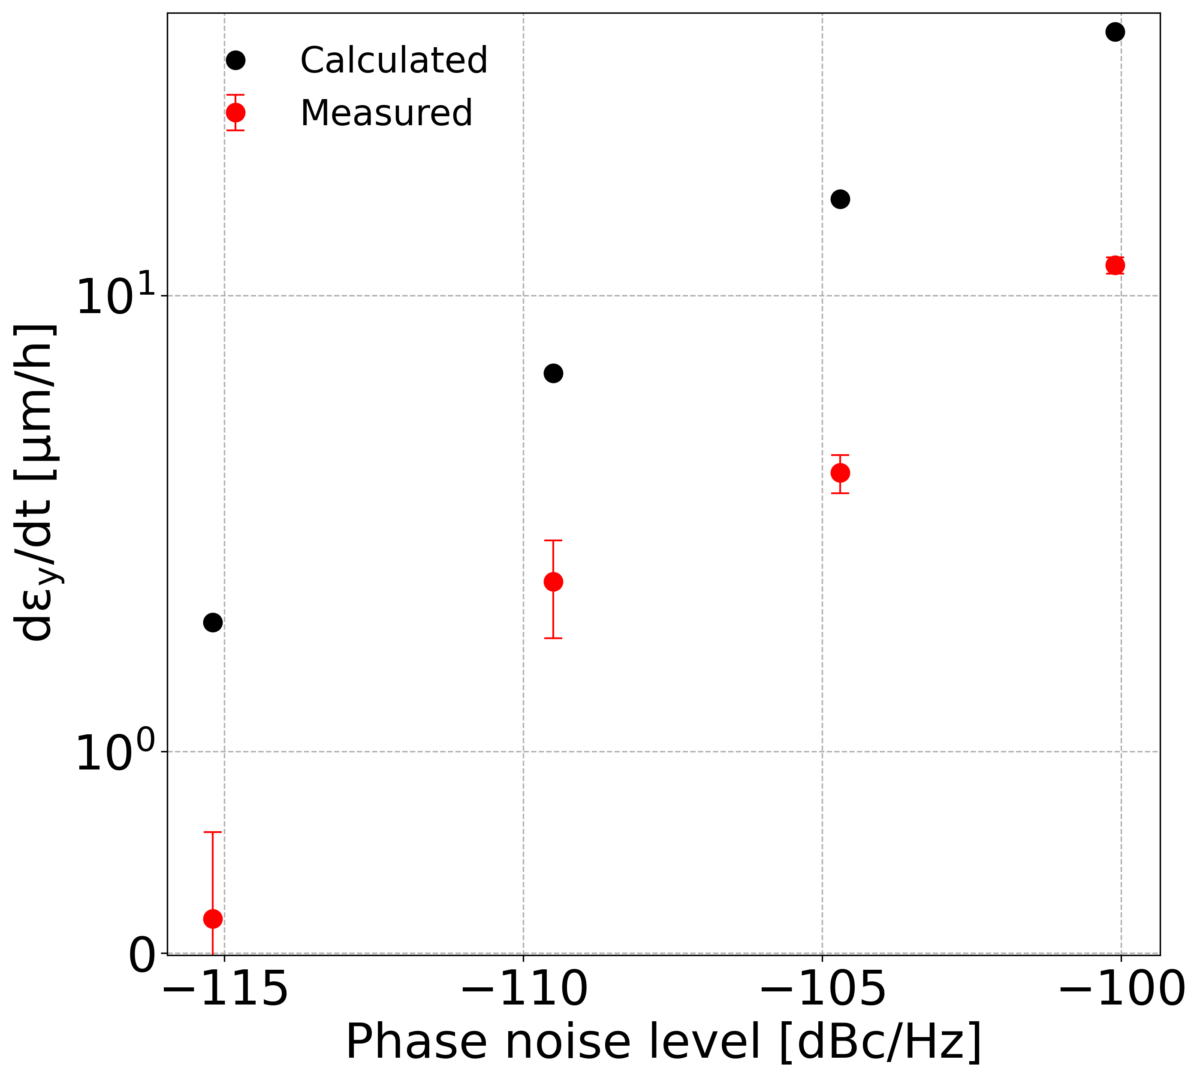
\includegraphics[width=0.7\textwidth]{images/Ch8/emit_V_background_subtracted_noise_scan.png}
       \caption{Summary plot of the emittance growth study with different noise levels injected in the RF system of CC1 in 2022. The vertical measured growth rate (red) and the expected growths from the theoretical model~\cite{PhysRevSTAB.18.101001} (black) are shown as a function of the different levels of applied phase noise. The error bars indicate the error of the linear fit on the emittance values (see Section~\ref{sec:emit_growth_meas_2018})}
       \label{fig:V_emit_growth_background_subtracted_noise_scan}
\end{figure}

From Fig.~\ref{fig:V_emit_growth_background_subtracted_noise_scan} it becomes evident that the measured emittance growth increases for higher noise levels as expected. Furthermore, it is observed that the theory systematically overestimates the measured growth rates. The averaged discrepancy over all noise levels, but the first one, is a factor 4: numerical values are given in Table~\ref{tab:cc_md_2022_noise_scaling}. In the computation of the average, the growth rates for the first noise level are not taken into account since the uncertainty of the corresponding measured growth is very big ($\sim 50\%$ of the emittance value itself).

\begin{table}[!hbt]
	\centering
   \caption{Comparison between the measured and the calculated transverse emittance growth rates for the different phase noise levels during the CC experiment of 2022. The analytical emittance growth rates were computed using Eq.~\eqref{eq:dey_pn} for rms bunch length of $4\sigma_t$=1.83\,ns.}
	\begin{tabu} to \textwidth { X[c,m] X[c,m] X[c,m] }
		&& \\[-6mm]
		\toprule \toprule
		\multicolumn{1}{c}{$\mathbf{10\,\boldsymbol{\log}_{10} \mathcal{L}(f)}$} &
      \multicolumn{2}{c}{\textbf{Growth rate [}$\mathbf{\boldsymbol{\mu}}$\textbf{m/h]}}  \\
		%\bottomrule
      \multicolumn{1}{c}{\textbf{[dBc/Hz]}} & \multicolumn{1}{c}{\textbf{\textbf{Measured}}} & \multicolumn{1}{c}{\textbf{Calculated}}  \\
      \midrule
      \multicolumn{1}{c}{-115.2}  & \multicolumn{1}{c}{0.17} & \multicolumn{1}{c}{1.64} \\
      
      \multicolumn{1}{c}{-109.5}  & \multicolumn{1}{c}{1.84} & \multicolumn{1}{c}{6.11} \\

      \multicolumn{1}{c}{-104.7}  & \multicolumn{1}{c}{3.25} & \multicolumn{1}{c}{18.44}  \\

      \multicolumn{1}{c}{-100.1}  & \multicolumn{1}{c}{12.11} & \multicolumn{1}{c}{53.19}  \\ 
      \arrayrulecolor{black}\bottomrule
	\end{tabu}
   \label{tab:cc_md_2022_noise_scaling}
\end{table}

To summarise, the first experiment of the experimental campaign with $\CC$s in 2022 has proved successful since:
\begin{itemize}
   \item The measured emittance growth was found to scale with the noise power as expected from the theory. 
   \item The measured growth rates were found to be systematically lower by the analytically expected values. This observation is in accordance with the experimental observations of the 2018 campaign and validates the reproducibility of the experiment. 
   \item The discrepancy between measured and theoretically expected values was found to be about a factor of 4, which is very close to the suppression factor of 3 which is expected from the PyHEADTAIL simulations with impedance (see Fig.~\ref{fig:pyheadtail_cc_impedance_2022_md_octupole_current} for $k_\mathrm{LOD}=0$).
\end{itemize}



\subsection{Results of CC Experiment B: sensitivity to amplitude-dependent tune shift}\label{subsec:cc_md_2022_octupole_scan}

The second part of the experiment aimed to validate that the beam coupling impedance suppresses the $\CC$ phase noise-induced emittance growth through the mechanism described in Section~\ref{sec:suppression_mechanism}. The strategy for this proof-of-concept expereiment was to measure the emittance growth for one level of phase noise (-104.7\,dBc/Hz or 3.4$\times 10^{11} \ \mathrm{rad^2/Hz}$) but for different octupole settings with the goal of reproducing the behavior shown in Fig.~\ref{fig:pyheadtail_cc_impedance_2022_md_octupole_current}. In the limited available time for the experiment performing the full scan on the octupole settngs was not feasible. Only five octupole strengths could be used, $k_\mathrm{LOD} = \pm 5 \ \mathrm{m^{-4}}, 10 \ \mathrm{m^{-4}}$ and $15 \ \mathrm{m^{-4}}$. The last value of octupole strength is expected to restore the growth rate to almost the values predicted by the theoretical model of T.~Mastoridis and P.~Baudrenghien~\cite{PhysRevSTAB.18.101001} ($\sim$ 20 $\mathrm{\mu m/h}$). For each setting the bunch evolution was recorded for about 20 minutes by acquiring repeated Wire Scanner measurements and then performing a linear fit. For the measurements of each setting a fresh bun was used such as the initial conditions are as close as possible. 

The individual measurements of the transverse emittance evolution for each octupole setting are illustrated in Fig.~\ref{fig:cc_md_2022_overview_plots_klod_scan}. Two main observations can be made by examining its subfigures. First, there is a clear sensitivity of the measured evolution of the vertical emittance on the octupole strength as expected from the PyHEADTAIL simualtions with the SPS transverse impedance model. The second observation is that a growth of $\sim 2-4 \ \mathrm{\mu m/h}$ is also observed in the horizontal plane. However, it does not seem to depend on the octupole strength. Both observations are also visualised in the summary plot of Fig.~\ref{fig:H_V_emit_growth_background_subtracted_octupole_scan}.

% location: /eos/user/n/natriant/2022/SPS_MDs_2022/cc_md_16May2022/roundA_online_analysis_ws/for_thesis
% script to plot: /afs/cern.ch/work/n/natriant/public/SPS_MDs_2022/cc_md_16May2022/ws_measurements 
\begin{figure}[htp]
   \centering
   \begin{subfigure}{.45\textwidth}
       \centering
       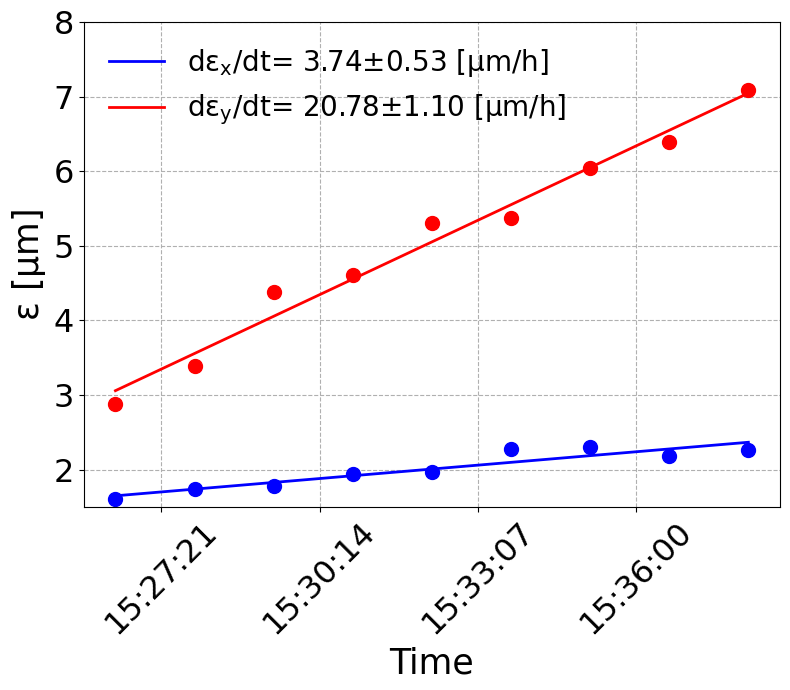
\includegraphics[width=.95\linewidth]{images/Ch8/emit_vs_time_Set1_coast6.png}  
       \caption{$k_\mathrm{LOD}=+15 \ \mathrm{1/m^{4}}$}
       \label{fig:cc_md_2022_coast6}
   \end{subfigure}
   \begin{subfigure}{.45\textwidth}
       \centering
       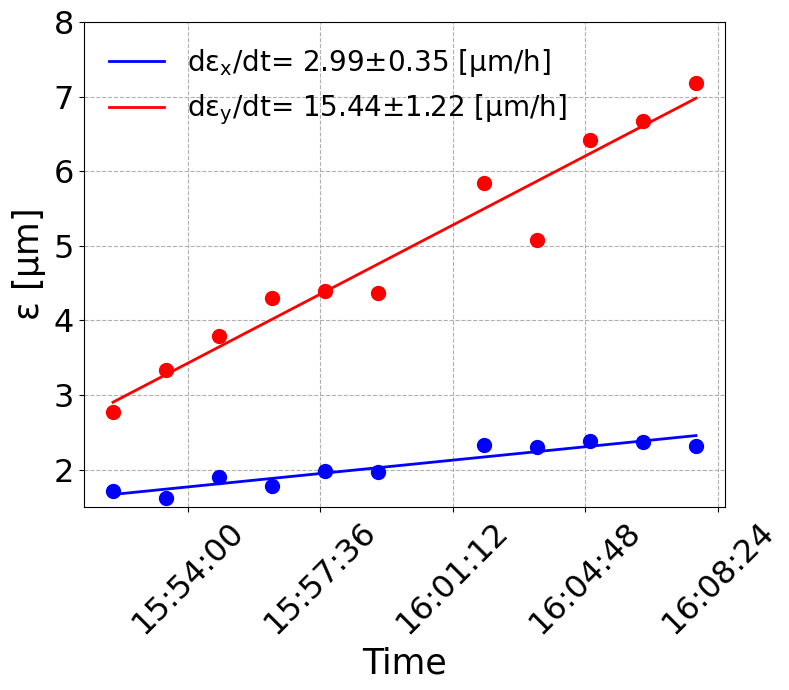
\includegraphics[width=.95\linewidth]{images/Ch8/emit_vs_time_Set1_coast7.png}  
       \caption{$k_\mathrm{LOD}=+10 \ \mathrm{1/m^{4}}$}
       \label{fig:cc_md_2022_coast7}
   \end{subfigure}
   \begin{subfigure}{.45\textwidth}
       \centering
       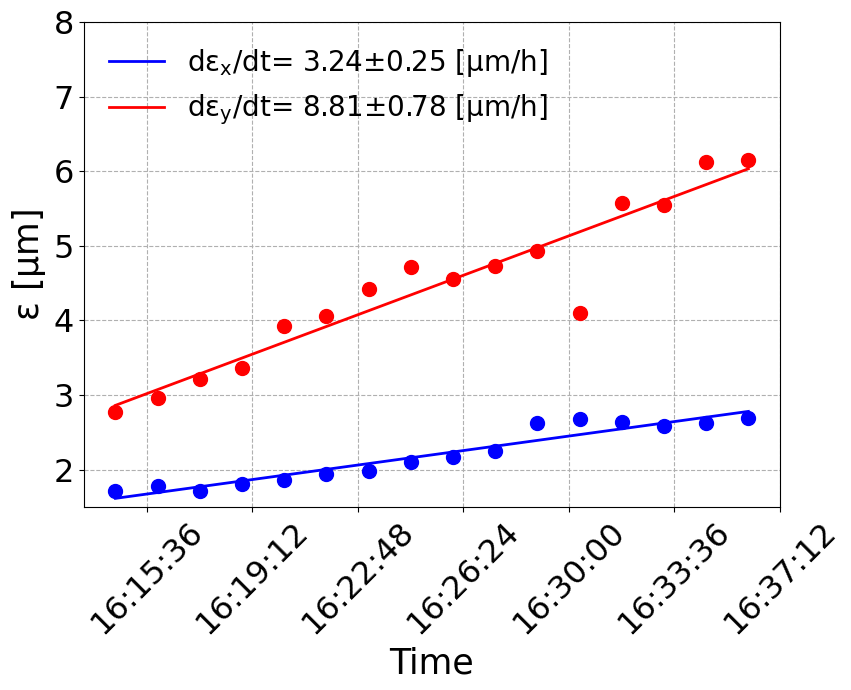
\includegraphics[width=.95\linewidth]{images/Ch8/emit_vs_time_Set1_coast8.png}  
       \caption{$k_\mathrm{LOD}=+5 \ \mathrm{1/m^{4}}$}
       \label{fig:cc_md_2022_coast8}
   \end{subfigure}
   \begin{subfigure}{.45\textwidth}
           \centering
           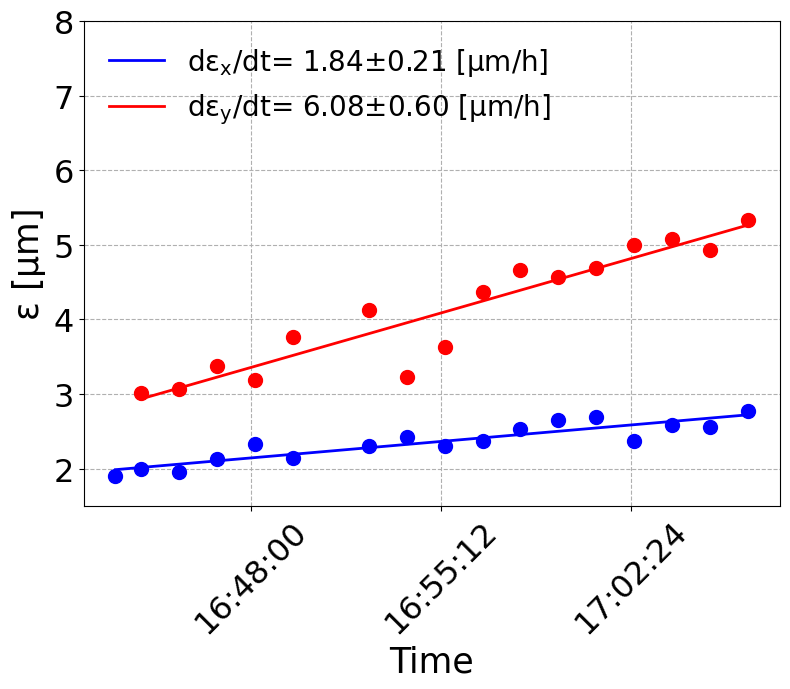
\includegraphics[width=.95\linewidth]{images/Ch8/emit_vs_time_Set1_coast9.png}  
           \caption{$k_\mathrm{LOD}=-5 \ \mathrm{1/m^{4}}$}
           \label{fig:cc_md_2022_coast9}
   \end{subfigure}
   \caption{Horizontal (blue) and vertical (red) emittance evolution of a single bunch during the CC experiment on May 16, 2022 driven by phase noise of -104.7\,dBc/Hz. The different octupole settings are displayed at the captions of each plot.}
   \label{fig:cc_md_2022_overview_plots_klod_scan}
\end{figure}

\textbf{Unstable bunch for strong negative octupole strength}\\
After the above presented measurements, there was an attempt to measure the emittance growth for $k_\mathrm{LOD}=-10 \ \mathrm{1/m^4}$. However, the bunch was found to be unstable in the vertical plane. The instability was first visible in the vertical beam profiles acquired with the Wire Scanners, where big tails started to appear. This is illustrated in Fig.~\ref{fig:instability_vertical_ws}. The instability was also observed in the turn by turn data acquired with the base band tune (BBQ) measurement system of SPS~\cite{Boccardi:1055568}, where the betatron oscillation amplitude appears to grow exponentially within a few seconds. This is illustrated in Fig.~\ref{fig:instability_BBQ_klod-15_4may2022}.

% Screenshot from MD logbook
\begin{figure}[!h]
   \centering         
   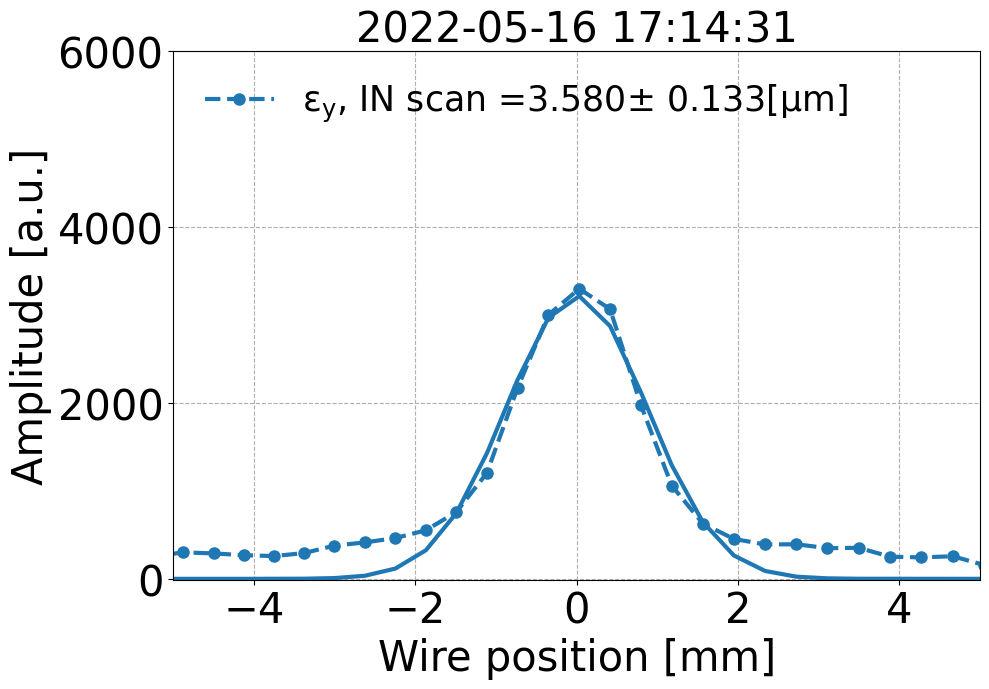
\includegraphics[width=0.7\textwidth]{images/Ch8/instability_41678.V_IN_OUT_ 17_14_31.png}
       \caption{Example measurement of the vertical profile during the experiment with phase noise of -104.7\,dBc/Hz injected in CC1 and $k_\mathrm{LOD}=-10 \ \mathrm{1/m^4}$. Due to the strong tails, the Gaussian fit (solid line) does not represent well the measured points (dots connected with the dashed line).}
       \label{fig:instability_vertical_ws}
\end{figure}


% Instability plotting: https://docs.google.com/presentation/d/1a1E84qGQi8w32hJTXj3IU7D5pAPSFc6oInAIOiykY04/edit#slide=id.g127f7feaac0_0_37
\begin{figure}[!h]
   \centering         
   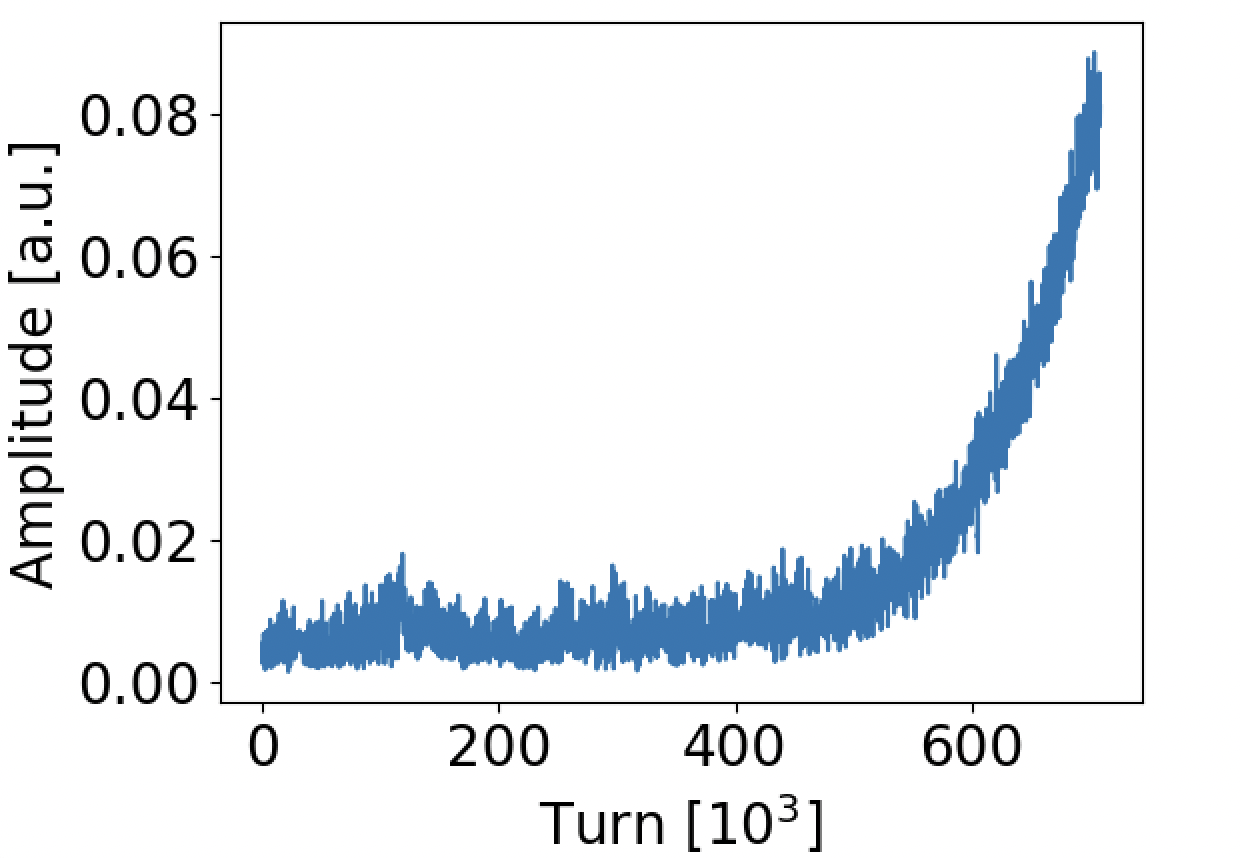
\includegraphics[width=0.7\textwidth]{images/Ch8/instability_klod-15_cc_md_4may2022.png}
       \caption{Example of the evolution of the oscillation amplitude in the vertical of the bunch centroid during the CC measurements for $k_\mathrm{LOD}=-10 \ \mathrm{1/m^4}$. This measurement is acquired with the BBQ instrument~\cite{Boccardi:1055568} and is a courtesy of X. Buffat (Email contact: xavier.buffat@cern.ch). \textcolor{red}{This figure is from the CC MD on May 4th. It needs to be updated with the corresponding figure from CC MD on May 16th 2022.} }
       \label{fig:instability_BBQ_klod-15_4may2022}
\end{figure}


The setting of almost zero linear chromaticity is the most likely explanation for this instability. As mentioned in the introduction of this chapter, the linear chromaticity was set to slightly above zero instead of 0.5-1.0 as it was requested due to miscommunication with the SPS operating team. This increased the probability of the chromaticity sliding to small negative values, which for machines like the SPS which operate above transition results to unstable bunches~\cite{collective_effects_cas_li}.

\textbf{Summary plot}\\
The measured emittance growth in both transverse planes is now plotted as a function of the different octupole strengths used in Fig.~\ref{fig:H_V_emit_growth_background_subtracted_octupole_scan}. The errorbars indicate the error of the linear fit on the emittance values during each coast. The background emittance growth observed in the SPS without any noise injected in the CC1 ($d\epsilon_x/dt$ = 0.81\,$\mathrm{\mu m/h}$ and $d\epsilon_y/dt$ = 0.84\,$\mathrm{\mu m/h}$) is subtracted from the measured values. 
%On this ground, it is reasonable to focus the rest of the analyisis in the vertical plane. 

Similarly, to the first part of the experiment (see Subsection~\ref{subsec:cc_md_2022_noise_scan}) the growth in the horizontal plane seems independent of the growth in the vertical. Furthermore, Fig.~\ref{fig:H_V_emit_growth_background_subtracted_octupole_scan} shows a clear dependence of the measured vertical emittance growth rate on the octupole strengths which appears similar to what is expected from the simulations. Therefore, the goal of the experiment is achieved as the experimental measurements confirmed the damping mechanism of the $\CC$ RF phase induced emittance growth from the transverse impedance. 

Additionally, for the measurements without powering on the octupoles, $k_\mathrm{LOD}=0$, the suppression factor is found to be $\sim$ 4-5 which is similar to what is expected from impedance.

The measured vertical emittance growth for the large octupole strength appears already slightly higher than the analytical prediction. This indicates that there is some uncertainty about the level of quantitative agreement which will be discussed further in the following paragraph which provides a direct comparison of the measured data with the simulation results.

% Plotting script: 2022/SPS_MDs_2022/cc_md_16May2022/roundA_online_analysis_ws/summary_plots/for_thesis/cc_md_octupole_scan_for_thesis.ipynb
\begin{figure}[!h]
   \centering         
   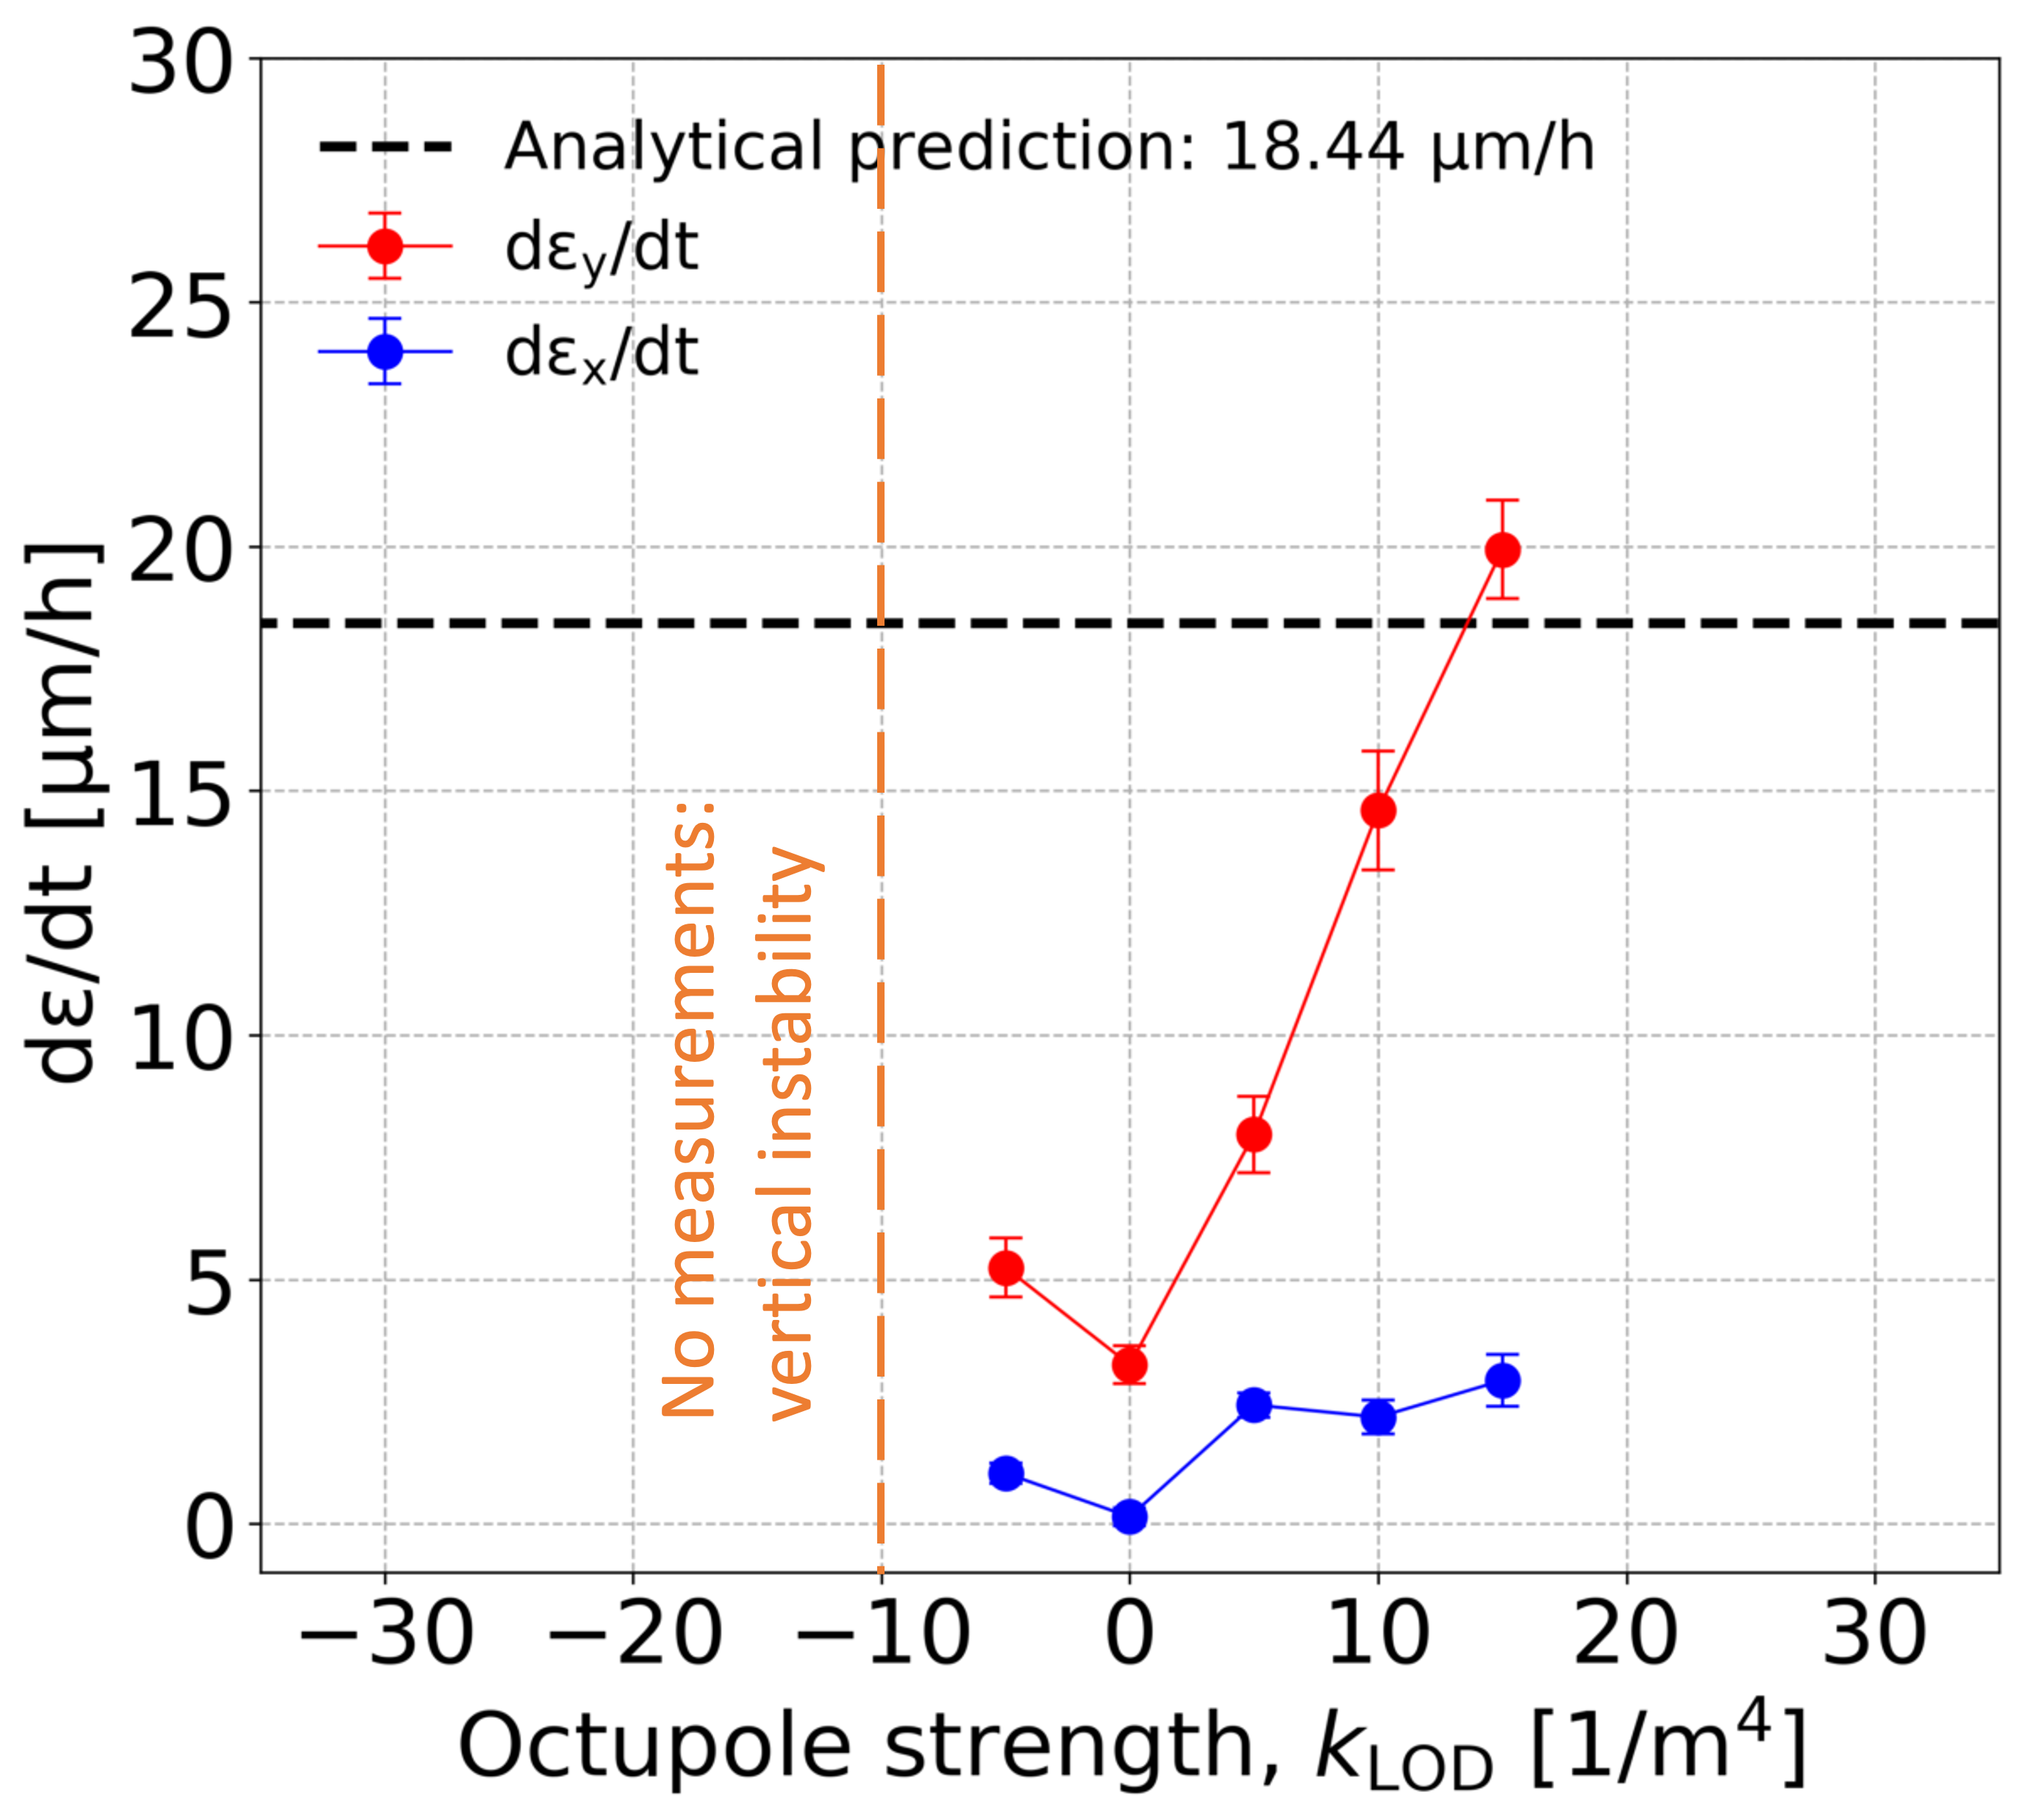
\includegraphics[width=0.7\textwidth]{images/Ch8/emit_H_and_V_octupole_scan_background_growth_subtracted_modified.png}
       \caption{Measured horizontal (blue) and vertical (red) emittance growth driven by phase noise of -104.7\,dBc/Hz injected in the RF system of CC1 for different octupole settings. The growth predicted from the analytical model without taking into account the impedance induced emittance growth suppression is $\sim$ 19\,$\mathrm{\mu m/h}$.}
       \label{fig:H_V_emit_growth_background_subtracted_octupole_scan}
\end{figure}

At this point, it should be highlighted that the degree of complexity of these studies is very high due to several reasons. First, the experiment aims to investigate the interplay of two effects: a) the $\CC$ noise-induced emittance growth and b) its suppression from impedance-induced effects, while for both of them the existing knowledge and previous experience are very limited.% for the first effect and non-existent for the second one. 
Second, preparational studies revealed that there is a high sensitivity of these effects and hence on the observables of the experiment on multiple parameters such as the bunch length, the intensity, the beam energy, the noise level, the $\CC$ voltage, the chromaticity, the tune spread, and the value of linear chromaticity. Third, a lot of uncertainties were introduced from the fact that the SPS did not operate in the usual mode.  In particular sources of uncertainties were: a) the $\CC$ that was switched ON b) the noise injected in the $\CC$ RF system c) the SPS that operates in stored mode and d) the octupoles operation out of their usual regime (high strengths/currents for a long time). % usually cycling.
Combining these factors, with the very limited machine time for the measurements, the fact that five data points were collected with very promising results which indicate a clear dependence on the octupoles' strength is a great success.


\textbf{Comparison of measurements against PyHEADTAIL simulations with the SPS impedance}\\

Figure~\ref{fig:cc_md_2022_measurement_vs_pyheadtail_simualtion} provides a direct comparison of the vertical emittance growth measurements with the simulation results from PyHEADTAIL including the SPS transverse impedance model (discussed in Fig.~\ref{fig:pyheadtail_cc_impedance_2022_md_octupole_current}). For the comparison, both measured and simulated rates are normalised with the corresponding analytical prediction (using Eq.~\eqref{eq:dey_pn}). 

% Plotting script: /eos/user/n/natriant/pyheadtail_data/final_for_thesis/2022_conditions/CC1/normalised_growth_vs_measurements/job0010b_plot_loadFromPickles_dey_scanOverAyy_NowakesVSwakes-octupoleSettings-Noconstraintaxy_plot_normalised.ipynb
\begin{figure}[!h]
   \centering         
   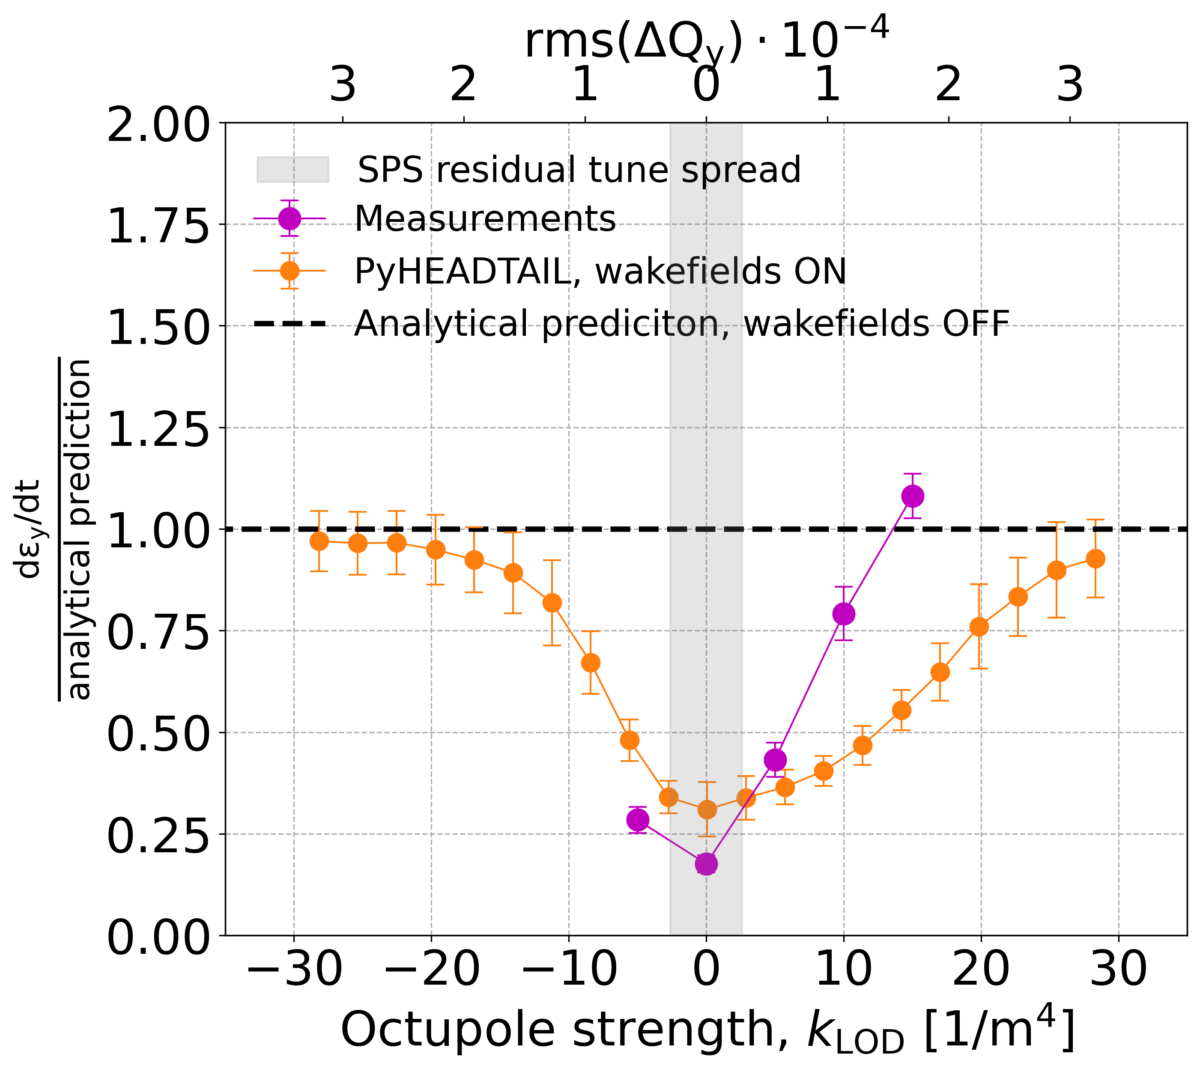
\includegraphics[width=0.7\textwidth]{images/Ch8/deyRates_sps_270GeV_PN1e-8_400MHz_SPS_NewWakesAllcontributions_appendWakes_y-plane_WakesONvsOFF_QpxQpy1_6D_Nb5e5_intensity3e10Scan_simulations_vs_measurements_magenta_new_legend.png}
       \caption{Measured horizontal (blue) and vertical (red) emittance growth driven by phase noise of -104.7\,dBc/Hz injected in the RF system of CC1 for different octupole settings. The growth predicted from the analytical model without taking into account the impedance induced emittance growth suppression is $\sim$ 19\,$\mathrm{\mu m/h}$.}
       \label{fig:cc_md_2022_measurement_vs_pyheadtail_simualtion}
\end{figure}

It can be seen, that there is a very good qualitative agreement of the measurements with the simulations confirming the damping mechanism from the impedance. Regarding the degree of quantitative agreement, there is some uncertainty, as already discussed above. Nevertheless, this is not surprising due to the uncertainty factors that were presented in the previous paragraph. Further studies, simulations, and measurements will be needed to investigate the quantitative agreement. One of the possible factors that could explain that quantitative is not yet obtained is the contribution from space charge which is not yet studied and it could affect the tune spread values. Space charge was not yet taken into account as its contribution is very small for the discussed experimental configurations. Nevertheless, the tune spread values in the regime of the studies are also very small, $10^{-6}-10{-4}$, which suggests that the space charge might have an important role. This can be investigated in simulations even though it is computationally challenging.

%\begin{itemize}
%   \item The contribution from space charge which is not yet studied and it could affect the tune spread values. 
 %  \item The fact that in the experiment the vertical emittances reached significantly larger final emittances than the 2\,$\mathrm{\mu m}$ that were considered in the simulations. Larger emittances mean larger action which eventually leads to a much larger tune spread than it was initially computed for this study. In other words, for the experimental conditions, $k_\mathrm{+15} \ \mathrm{1/m^4}$ the resulting incoherent spectrum might be sufficient for the coherent tune to lie inside it. %Linear, non-linear?
%\end{itemize}

As the objective of the experiment and this thesis, in general, are already achieved, these studies are considered complementary. Therefore, they are not performed yet nor they will be presented here, due to time restrictions for the completion of this thesis. 

%\subsection{Conclusions and outlook}\label{subsec:conlusions_ch8_cc_md}
%The experimental results of the additional experimental campaign with $\CC$s in SPS that took place on May 16, the year 2022 were presented in this section. The subject of the studies was the investigation of the $\CC$ noise-induced emittance growth and in particular its suppression from the beam transverse impedance. The two main objectives were a) to reproduce the scaling of the emittance growth with noise power that was observed in 2018, and b) to confirm that the beam coupling impedance can effectively suppress the $\CC$ phase noise-induced emittance growth. For the latter, the strategy was to reproduce the strong dependence of the suppression factor on the amplitude-dependent tune shift as obtained from PyHEADTAIL simulations with the SPS impedance model.

%Despite the limited available machine time and the numerous uncertainties introduced by the SPS operation outside of its usual mode, the experiment was proved successful. In particular, the experiment demonstrated that the vertical emittance increased for stronger noise in agreement with the observables of 2018 and the expectations from the available analytical model of T.~Mastoridis and P.~Baudrenghien. Moreover, the measurements showed good qualitative agreement with the expected impact of impedance and amplitude detuning: they represent a proof of concept for the mechanism of emittance growth suppression from the transverse impedance. Further studies, simulations (e.g. contribution of space charge), and measurements (e.g. varying octupole strengths over a larger range, impact of linear chromaticity, and the sensitivity to transverse instabilities), will be needed to refine the experimental observations and to investigate the quantitative agreement. 




\section{Experiment with dipole noise}\label{sec:coast_md_damper_2022}
% Presentation with the results:  https://docs.google.com/presentation/d/1C-3FPNUrUUiOFol2bdMlTqf1ZlGVamcZXjf-b4lYlUM/edit#slide=id.g1301694a1dd_0_139
The second proof-of-concept experiment for the damping mechanism from the transverse impedance was conducted the night after the $\CC$ experiments described in the previous section. The emittance growth was induced by the beam damper acting as a pure dipolar noise source. This simplified the experimental procedure for two main reasons. First, there were no limitations and uncertainties introduced by the $\CC$ operation. Secondly, activating the beam damper does not require the teams which operate the $\CC$s and inject artificial noise into their RF system and thus less coordination. This mitigates the restrictions on finding an available slot for this experiment which eventually was squeezed during the night shift after the measurements with $\CC$s. % cryo team not needed

The strength of the damper kick was not calibrated and therefore the analytical expected emittance growth could not be computed. Nevertheless, the objective was to reproduce the strong dependence on the amplitude detuning which was presented in Fig.~\ref{fig:study_5_dipole_noise}). To this end, the same procedure with the second part of the $\CC$ experiment was followed: the emittance growth was measured in coast for constant strength of the noise excitation in the vertical plane but for different octupole settings. The beam and machine parameters are summarised in Table~\ref{tab:machine_beam_param_2022}. The only update was that the linear chromaticity was corrected to $Q^\prime_{x,y}$ = 1.3 in both transverse planes to avoid instabilities due to possible shift of chroma to negative values (see Figs.~\ref{fig:instability_BBQ_klod-15_4may2022} and~\ref{fig:instability_vertical_ws}). 

The experiment lasted from about 23:50 on the 16th of May, 2022, until about 04:00 on the 17th of May, 2022. Even though the available machine time was $\sim$4 hours, only seven octupole strengths could be tested: $+25, +15, +10, +5, 0, -15, -7.5 \ \mathrm{1/m^4}$. The reason is that one of the SPS quadrupole magnets tripped around 01:00 disabling the option for operation in coast, till around 03:00 when the quadrupole magnet got back working.

For each octupole setting, the bunch evolution was recorded for about 10 minutes by acquiring repeated measurements with the Wire Scanners (the same instruments were used for the $\CC$ experiment earlier that day). The short duration of the measurements was a result of the strong noise excitation which resulted to a clear linear growth of the vertical emittance which reached quickly large values. This can be seen in the individual measurements of the transverse emittance evolution for each octupole setting which are presented in the Appendix... For the measurements of each setting a fresh bunch was injected. 


\textbf{Summary plot}\\
% no bacgkorund growth is subtracted here. It was not measured. Sensitivity very small as we are dealing with very strong emittance growth. Impact of backgorund growth is insignificant.
The experimental results are summarised in Figure~\ref{fig:coast_dipole_noise_damper_md_2022_measurement}. The measured horizontal and vertical emittance growth are plotted as a function of the different octupole strengths with blue and red colors respectively. The error bars indicate the error of the linear fit on the emittance values during each coast. The background emittance growth without any noise excitation from the damper was not measured and thus is not subtracted from the displayed values. However, the impact of the background growth (usually measured to be between 0.5-1$\mathrm{\mu/h}$ in both transverse planes) is insignificant for the emittance growth rates of this study ($ > 10 \ \mathrm{\mu/m}$).
 

The emittance growth observed in the horizontal plane appears to be independent of the growth in the vertical, agreeing with the observations during the $\CC$ experiment (see Section~\ref{sec:cc_md_2022}). 

In the vertical plane, there is a clear dependence of the measured emittance growth on the strength of the octupoles as expected (see Fig.~\ref{fig:study_5_dipole_noise}). To this end, this experiment has been proved also successful since the results confirm the damping mechanism of the emittance growth from dipolar noise excitation by the beam transverse impedance. However, it is not clear if the used octupole strength was sufficient to get out of the suppression region. More data points with higher octupole strength would be needed. This is planned to be tested in dedicated future experiments.

Last, it is worth commenting that, unlike the $\CC$ experiment that was conducted earlier that day, no vertical instability was observed in this experiment. It appears, that correcting to $Q^\prime_{x,y}$ = 1.3 was an effective way of avoiding it.
  

% Plotting script: /eos/user/n/natriant/2022/SPS_MDs_2022/coast_md_damper_16May2022/summary_plots/create_pickle_for_octupole_scan.ipynb
\begin{figure}[!h]
   \centering         
   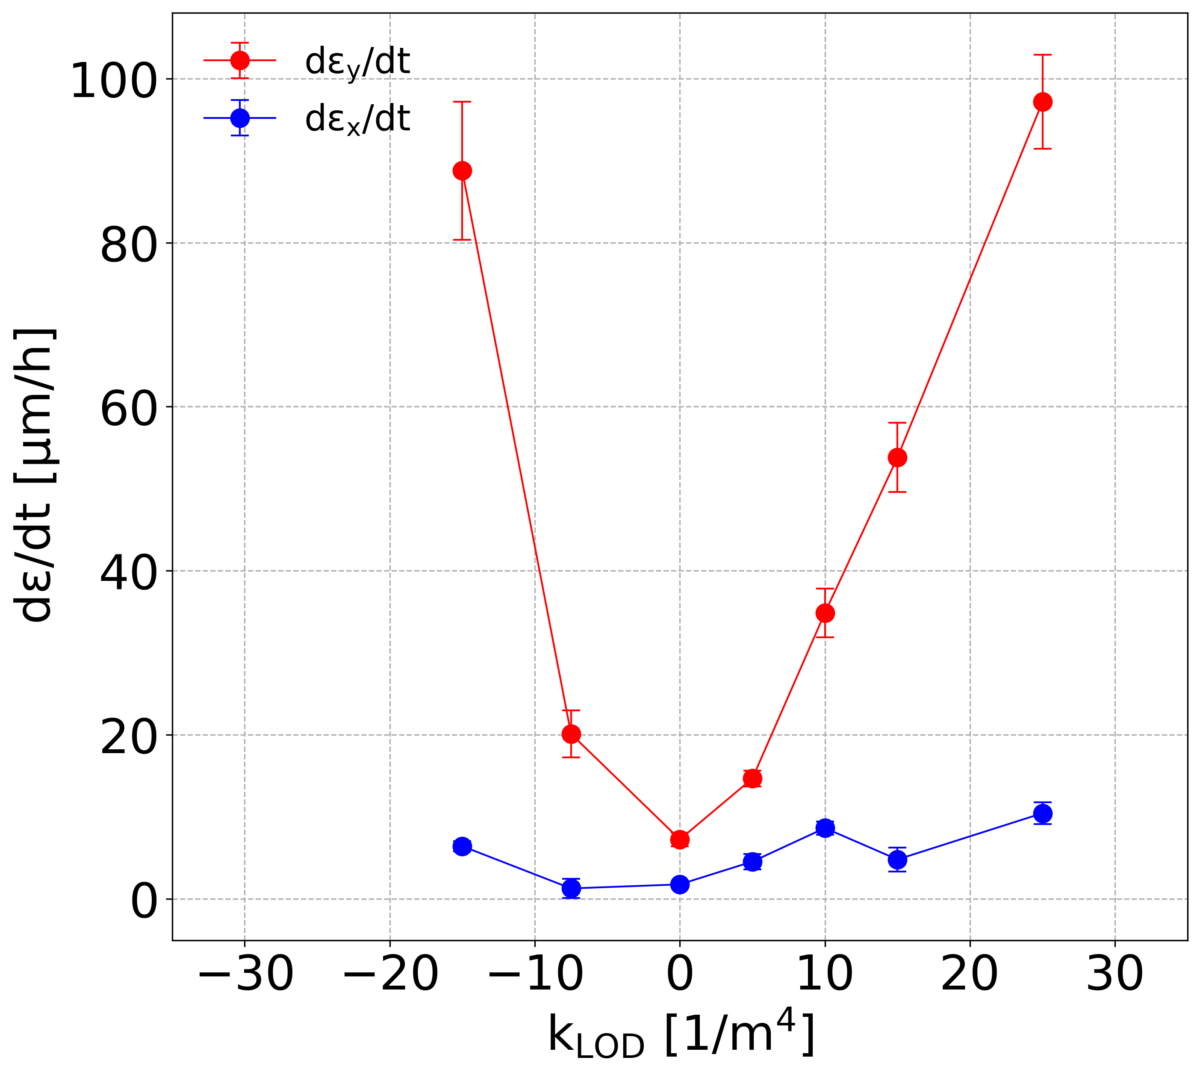
\includegraphics[width=0.7\textwidth]{images/Ch8/emitGrowth_H_V_dipole_noise_damper_md_measurements.png}
       \caption{Measured horizontal (blue) and vertical (red) emittance growth driven by dipole noise introduced with the SPS beam kicker in the vertical plane for different octupole settings.}
       \label{fig:coast_dipole_noise_damper_md_2022_measurement}
\end{figure}

\textbf{Underlying theory}\\
It is worth mentioning that the simulation studies and experimental results (from 2018 and 2022) presented in this thesis, motivated the development of a theoretical description for the suppression of the noise-induced emittance growth from the beam transverse impedance. The theory was recently developed by the colleague X.~Buffat\footnote{Email contact: xavier.buffat@cern.ch} and it is presented in in Refs.~\cite{Buffat:2022dac} and~\cite{van_kamper_presentation_xavier_theory}. 

The theory developed is a simplification of the approach of Y.~Alexahin (in the context of beam-beam interactions)~\cite{Alexahin:485304}. In particular, X.~Buffat, using the Van Kampen mode approach~\cite{VANKAMPEN1955949}, adapted Y.~Alexahin's approach for configurations featuring linear detuning and a complex tune shift from a collective force. 

% This paragraph is modified from the conclusions in Xavier's paper.%
It was shown that the emittance growth driven by an external noise source can be significantly reduced by a collective force. To observe the suppression a damping force is necessary. The suppression is enhanced in configurations where the real tune shift is larger than the spread of the betatron frequencies i.e. the coherent mode emerges from the incoherent spectrum~\cite{Buffat:2022dac}.

This theory supports the studies presented in this thesis. It also explains the asymmetry in the dependence of the emittance growth suppression for positive and negative detuning coefficients observed in PyHEADTAIL simulations (see Chapter~\ref{Ch:suppression_impedance}). Moreover, it was used to fit the experimental data measured during the experiment with dipole noise with very promising results.
% The figures is a screenshot from the plots of the following presentation: https://indico.cern.ch/event/1170242/contributions/4915101/attachments/2476586/4250387/2022-07-07_crabMD-expanded.pdf
%\begin{figure}[!h]
%   \centering         
%   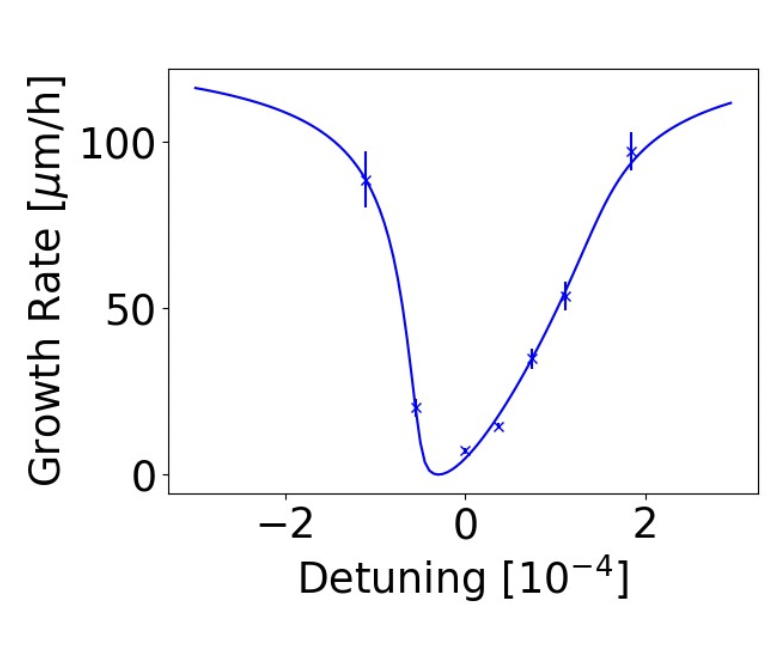
\includegraphics[width=0.6\textwidth]{images/Ch8/fit_van_kamper_damper_md_data_xavier.png}
%       \caption{Fit of Eq... to the measured emittance growth rates (points) during the experiment with a dipolar noise source. This figure is a courtesy of X.~Buffat.}
%       \label{fig:fit_van_kamper_xavier}
%\end{figure}


%\subsection{extra}
%check the  detuning with amplitude
%https://docs.google.com/presentation/d/1yaGKJ20O-jVg0R3bdj62l5VzltwjBBHtphKq5HI9xrY/edit#slide=id.g104dd3ff735_0_184


%\section{Bunch length measurements} --> Moved in the appendix
% https://docs.google.com/presentation/d/1cqXVwsXoorYqU9Td0qiFDBcyAn9XrNLmL_kvYOj61yU/edit#slide=id.g129fd6f84c7_1_5


\section{Conclusions and outloook}\label{sec:Ch8_conclusions}
The experimental results of the additional experimental campaign with $\CC$s in SPS that took place on May 16, the year 2022 were presented in this section. The subject of the studies was the investigation of the $\CC$ noise-induced emittance growth and in particular its suppression from the beam transverse impedance. The two main objectives were a) to reproduce the scaling of the emittance growth with noise power that was observed in 2018, and b) to confirm that the beam coupling impedance can effectively suppress the $\CC$ phase noise-induced emittance growth. For the latter, the strategy was to reproduce the strong dependence of the suppression factor on the amplitude-dependent tune shift as obtained from PyHEADTAIL simulations with the SPS impedance model.

Despite the limited available machine time and the numerous uncertainties introduced by the SPS operation outside of its usual mode, the experiment was proved successful. In particular, the experiment demonstrated that the vertical emittance increased for stronger noise in agreement with the observables of 2018 and the expectations from the available analytical model of T.~Mastoridis and P.~Baudrenghien. Moreover, the measurements showed good qualitative agreement with the expected impact of impedance and amplitude detuning: they represent a proof of concept for the mechanism of emittance growth suppression from the transverse impedance. Further studies, simulations (e.g. contribution of space charge), and measurements (e.g. varying octupole strengths over a larger range, impact of linear chromaticity, and the sensitivity to transverse instabilities), will be needed to refine the experimental observations and to investigate the quantitative agreement. 

Last, additional measurements with emittance growth driven by a pure dipolar noise source (the beam transverse damper) clearly demonstrated the dependence of the emittance growth suppression: supporting the results with the $\CC$ noise and validating once more the mechanism of the suppression of the emittance growth by the beam transverse impedance. 

% From IPAC
%During the SPS CC tests in 2018, it was found that theoretical calculations of the transverse emittance growth from CC RF noise overestimated the measurements by a factor 4 (Chapter~\ref{Ch:2018_analyisis}). Simulations with PyHEADTAIL indicated that the discrepancy might be explained by impedance effects, in particular when the coherent tune is shifted outside of the incoherent spectrum (Chapter~\ref{Ch:suppression_impedance}). The simulations also indicated that the suppression is related to the dipole motion (mode 0) and a strong dependence on amplitude detuning: this was tested experimentally in the SPS in 2022. 

%The emittance growth studies took place first in the presence of $\CC$ RF phase noise and after in the presence of pure dipolar noise excitation from the beam transverse damper. The results from both expereiments show good qualitative agreement with the expected impact of impedance and amplitude detuning: they represent a proof of concept for the mechanism of emittance growth suppression from transverse impedance. 


%The noise kicks from the transverse damper were not calibrated so a quantitative comparison with the simualtion results was not feasible. For the experiment where the emittance growth was driven by $\CC$ the quantitative agreement was 


%The objective of the experimental campaign with emittance growth studies se in the SPS in 2022 was to validate experimentally the $\CC$ RF noise induced emittance growth suppression mechanism from the beam transverse impedance as suggested by PyHEADTAIL simualtions. The simualtions suggested that the meachanism is related to the dipole motion (mode 0) to this end two experiments took place. In the first, the emittance growth was driven by $\CC$ RF phase noise (like in 2018), while in the second it was driven by the beam transverse noise which provided a pure dipolar noise excitation.

%This would a) explain the 

%IPAC?

